% !TeX spellcheck = en_US
\documentclass[11pt, a4paper, english, hidelinks, twoside, openright]{report}
%Fixes the "no room for \count error"
% @see http://tex.stackexchange.com/questions/186588/what-does-the-etex-package-do-exactly
\usepackage{etex}
\usepackage{babel}
% All pages with no text (generated in order to have chapters start on odd numbered pages) will be completely empty.
\usepackage{emptypage}	
\usepackage{cite}
\usepackage{microtype}
\usepackage[utf8]{inputenc}
\usepackage[T1]{fontenc}
\usepackage{graphicx}
\usepackage{listings}
\usepackage[margin=1in]{geometry}
\usepackage[ddmmyyyy]{datetime}
\usepackage[dvipsnames]{xcolor}
\usepackage{mathtools}
\usepackage{amsfonts, amsmath}
\usepackage{mathptmx}
\usepackage{caption}
%For big letters when starting a new chapter
\usepackage{lettrine}			
\usepackage{enumitem, enumerate}
\usepackage[all]{xy}
\usepackage{todonotes}
\usepackage{array}
\usepackage{longtable}
\usepackage{pgfplots}
\usetikzlibrary{positioning}
\usepackage{url}
\usepackage{listings}
\usepackage{bm}
\usepackage[useregional]{datetime2}
\usepackage[space]{grffile}
\usepackage{multicol}
\usepackage{etoolbox}
\usepackage{relsize}
\usepackage{subfig, etoolbox}
\usepackage{float}
\usepackage{pdfpages}
\usepackage[newfloat]{minted}
\usepackage{csvsimple}
\usepackage{fixmath}
\usepackage{booktabs}
\usepackage{hyperref}
\usepackage{amsthm}
%cleveref must be loaded after hyperref
\usepackage{cleveref}				
\usepackage{fancyhdr}
\usepackage{pdfpages}

%Disable pageanchors for the pages before the introduction. It will be turned on before inlcusion of the introduction. It will fix the 'same destination' error, where two pages have the same page number (although some one page number is not shown)
\hypersetup{pageanchor=false}	

%%%%%%%%%%%%%%%%%%%%%%%%%%%%%%%%
% New commands and definitions %
%%%%%%%%%%%%%%%%%%%%%%%%%%%%%%%%
	
%%%%%%%%%%%%%%%
% Custom Font %
%%%%%%%%%%%%%%%
\pdfmapfile{=mtpro2.map}
\usepackage[lite, subscriptcorrection]{mtpro2}

%%%%%%%%%%%%%%%%%%%%%%
% Royal Intials Font %
%%%%%%%%%%%%%%%%%%%%%%
\input RoyalIn.fd
\newcommand*\initfamily{\usefont{U}{RoyalIn}{xl}{n}}

%%%%%%%%%%%%%%%
% Definitions %
%%%%%%%%%%%%%%%

\DeclarePairedDelimiter\abs{\lvert}{\rvert}
% Swap the definition of \abs* ,so that \abs
% resizes the size of the brackets, and the 
% starred version does not.
\makeatletter
\let\oldabs\abs
\def\abs{\@ifstar{\oldabs}{\oldabs*}}
\makeatother

%%%%%%%%%%%%
% Settings %
%%%%%%%%%%%%
\graphicspath{{img/}}
\captionsetup{hypcap=false}
%Supress PDF inclusion warnings. If it throws an error, you must upgrade MikTex packages.
\pdfsuppresswarningpagegroup=1
\pgfplotsset{compat=1.13}

%http://stackoverflow.com/questions/491904/how-do-i-remove-blank-pages-coming-between-two-chapters-in-appendix
\let\cleardoublepage\clearpage 	

%%%%%%%%%%%%%%%%%%%%%%%%%%%%%%%%%%%%%%%%%%%%%%
% Minted Source Code Spanning Multiple Pages %
%%%%%%%%%%%%%%%%%%%%%%%%%%%%%%%%%%%%%%%%%%%%%%%%%%%%%%%%%%%%%%%%%%%%%%%%%%%%%%%%%%%%%%%
% @see http://tex.stackexchange.com/questions/254044/caption-and-label-on-minted-code %
%%%%%%%%%%%%%%%%%%%%%%%%%%%%%%%%%%%%%%%%%%%%%%%%%%%%%%%%%%%%%%%%%%%%%%%%%%%%%%%%%%%%%%%
\newenvironment{code}{\captionsetup{type=listing}}{}
\SetupFloatingEnvironment{listing}{name=Listing}

%Otherwise geometry resets everything
\makeatletter 
\Gm@restore@org
\makeatother

\captionsetup[figure]{position=b}
\captionsetup[subfigure]{position=b}
\captionsetup[subtable]{position=t}

\setlength{\itemsep}{0cm}
\setlength{\voffset}{0cm}
\setlength{\headheight}{0cm}
\setlength{\topmargin}{0cm}
%Superscripts in tabular
\setlength{\extrarowheight}{3pt} 
\setlength{\arraycolsep}{4pt}
\lstset{basicstyle = \footnotesize, breaklines = true}

%%%%%%%%%%%%%%%%%%%%%%%%%%%%%%%
% Bibliography in two columns %
%%%%%%%%%%%%%%%%%%%%%%%%%%%%%%%
\patchcmd{\thebibliography}
{\list}
{
% Add Bibliography as an entry in Table of Contents
\csname phantomsection\endcsname\addcontentsline{toc}{chapter}{\bibname}	
\begin{multicols}{2}\smaller\list
}
{}
{}
\appto{\endthebibliography}{\end{multicols}}

%%%%%%%%%%%%
% Commands %
%%%%%%%%%%%%
\newcommand{\source}[1]{\caption*{Source: {#1}} }

%%%%%%%%%%%%%%%%%%%%%%%%
% Header custimization %
%%%%%%%%%%%%%%%%%%%%%%%%
\pagestyle{fancy}
% Set both header and footer to nothing
\fancyhf{}
\renewcommand{\headrulewidth}{0pt}
%Changes placement of page numbers to: Right on Even pages, Left on Odd pages

\fancyfoot[RE, LO]{\thepage}	

%%%%%%%%%%%%%%%%%%%%%%%%%%%%%%%%%%%%
% Redefinition of \Chapter command %
%%%%%%%%%%%%%%%%%%%%%%%%%%%%%%%%%%%%
\makeatletter
\renewcommand\chapter{\if@openright\cleardoublepage\else\clearpage\fi
                    \thispagestyle{fancy}%
                    \global\@topnum\z@
                    \@afterindentfalse
                    \secdef\@chapter\@schapter}
\makeatother

%%%%%%%%%%%%%%%%%%%%%%%%%%%%%
% Redefine \cleardoublepage %
%%%%%%%%%%%%%%%%%%%%%%%%%%%%%
%Removes the page numbers on empty pages
\makeatletter
\renewcommand*{\cleardoublepage}{\clearpage\if@twoside \ifodd\c@page\else
\hbox{}%
\thispagestyle{empty}%
\newpage%
\if@twocolumn\hbox{}\newpage\fi\fi\fi}
\makeatother


%%%%%%%%%%%%%%%%%%%%%%%%%%%%%
% Bachelor Thesis Structure %
%%%%%%%%%%%%%%%%%%%%%%%%%%%%%
\begin{document}
\input{front/"Title Page"}
\cleardoublepage
% !TeX spellcheck = en_US
% !TeX root = ../BachelorThesis.tex
\begin{abstract}
	Multiple sclerosis (MS) is a disease where the day quality of a patient can vary a lot.
	Therefore, it is hard to predict whether upcoming days will be `good' or `bad' days.
	By identifying relevant biomarkers for patients using data from wearables, we might be able to predict this day quality.
	These predictions can be used to get more personal advice on and insight in MS.
	
	After we identified relevant biomarkers using literature research, we chose to research the following three biomarkers: Two-Minute Walk Test (2MWT), resting heart rate (RHR) and sleep duration.
	Using statistical analysis on each of these biomarkers, we investigated the correlation between the data belonging to this biomarker and the rating of the day after indicated by each of the participants.
	Although the period in which we gathered the data was reasonable, the amount of data was lower and of lesser quality than expected.
	This was especially the case for data that only could be gathered when participants entered specific information in the application that we used during our experiment, 
	In the end, we did not find any evidence for a relation between each individual biomarker and the day rating for the next day.
	We did find that the process of gathering data from research subjects should preferably be fully automated (if possible).
	This is because participants tend to forget or ignore instructed tasks, although these tasks are essential for the data that will be used in research.
	Participant adherence was one of the major factors impacting the quality of our data and should be taken into account in future research.
\end{abstract}

\cleardoublepage
% !TeX spellcheck = en_US
% !TeX root = ../BachelorThesis.tex
\renewcommand{\abstractname}{Acknowledgements}
\begin{abstract}
	I would like to thank my supervisor Tom Heskes for his time and support during my research. 
	I would also like to thank Bram den Teuling for granting me the opportunity to write my thesis at Orikami and to work on this interesting topic. 
	Finally I would also like to thank my parents for their never ending support.
\end{abstract}

\microtypesetup{protrusion=false}
\tableofcontents
\microtypesetup{protrusion=true}
\hypersetup{pageanchor=true}

% !TeX spellcheck = en_US
% !TeX root = ../MS_analysis_thesis.tex
\chapter{Introduction}\label{introduction}

\section{Motivation and Research Questions}
\lettrine[lhang = 0.4, findent=-60pt, lines=7]{\textbf{
		\initfamily \fontsize{40mm}{40mm} \selectfont M
		\normalfont}}{ultiple sclerosis (MS)}
 is a long lasting disease that affects approximately 1 in 1000 people in the Netherlands.
MS is a disease of the central nervous system, resulting in disrupted communication between the brain and other parts of the body.
In MS, the insulating covers of nerve cells, called myelin, are damaged.  
The symptoms range from reduced vision to muscle weakness. 
Depression is also a common symptom of MS.

There are four different courses for MS \cite{lublin2014defining}.
The most common course is called relapsing-remitting MS (RRMS).
RRMS is characterized by attacks, also called relapses, followed by periods of partial or complete recovery (remissions).
These periods of attacks and recovery can, especially for MS patients with RRMS, result in good and bad days.
Because there is no cure for MS, treatment tries to prevent and improve the recovering from these attacks.

Orikami is currently developing an app called DiaPro MS. 
Participants in the pilot experiment of this app will receive activity trackers. 
MS patients will wear these activity trackers for a period of two months.
During this period, the activity tracker will capture biomarkers like heart rate, blood pressure, steps walked and the amount of sleep during the day.
Together with the data gathered from filled in questionnaires, these biomarkers could be used to predict good and bad days for MS patients.

This thesis will focus on how to capture reliable biomarkers using wearables and try to overcome any difficulties faced during the pilot. 
It will provide more insight in the process of using wearables in research and how the captured data can be used for analysis.
This is useful when the experiment will be done on a much larger scale. 

The main question of this research is: \textbf{which biomarkers, captured by activity trackers, are possibly useful for the prediction of good and bad days for MS patients? }
To answer this question, we need to answer the following subquestions:
%
\begin{itemize}
	\item[$\star$] What is the reliability and validity of biomarkers captured by activity trackers?
	
	\item[$\star$] How are biomarkers measured?
	
	\item[$\star$] How can biomarkers be used as an indicator of health?
\end{itemize}
%

\section{Related Work}
In this section, we will look at literature that is related to making predictions of the quality of upcoming days for people having MS.
As we have seen in our previous section, MS is a complex disease with several processes playing role in the course of it.
Biomarkers are used to get a measurement of the current state or condition of a person.
This is done by measuring indicators.
Traditionally, biomarkers are substances measured in body fluids, saliva and blood.
Current research is continuously finding new relevant biomarkers for MS.
Several papers exist that give an up to date overview of current biomarkers \cite{bielekova2004development, katsavos2013biomarkers}. 
These biomarkers can be very useful in distinguishing several subgroups of MS.
New types of biomarkers like stress and neurodegeneration (the loss of neurons) are being explored.
By exploring these biomarkers, researchers speed up the process of using these biomarkers in clinical practice.
With the introduction of the activity trackers and smart watches, more biomarkers can be measured easily.
Although research related to the reliability and validity of the measurements from these devices is still being conducted, the devices are currently being used in the research field.

By using measurements of heart rate, exercise capability (2MWT) and more we could give a patient more insight in his upcoming days.
Prediction of quality of life in multiple sclerosis has been researched before. 
Health-related quality of life (HQOL) is used to determine an individual's well-being. 
This can be affected over time, depending on the disease or other conditions.
For MS patients, HQOL is poor.
In \cite{benedict2005predicting}, several predictors (depression and self-reported fatigue) were considered simultaneously.
In a group of 120 MS patients and in a control group of 44 people, HQOL was measured.
It was found that MS patients reported lower HQOL compared to the control group.
Depression and fatigue were the primary contributors to these results.
This confirms the results of previous studies, where a strong relation was found between depression and HQOL in MS.
A limitation of self reports is that the results are not objective: they depend on the mood of the patient.
As we can see in previous studies, the prediction of upcoming days is something that remains unaddressed.

In \cite{galea2013web}, a web-based calculator was made for MS patients.
This calculator was able to give estimates of the progression of the disease.
By letting the user provide individual patient characteristics like disease course, number of attacks in the last two years and the age on which the first MS symptoms appeared, the calculator tried to find the best matching patients in a database.
Using these matched patients, MS related prognoses were calculated for this specific individual having MS. 
One of these prognoses was the time it would take for the patient to transition from RRMS to secondary progression MS (SPMS).
These predictions where then compared to the predictions of 17 MS specialist neurologists.
They were asked how long it would take for the presented MS patients to reach a value of 10 on the expanded disability status scale (EDSS) after their first MS symptoms.
This means death due to MS.
The predictive accuracy was measured using the Brier Score, which is a score function that measures the accuracy of probabilistic predictions. 
A score of 0 indicates perfect accuracy, while 0.5 indicates the same accuracy as chance.
The Evidence-Based Decision Support Tool in Multiple Sclerosis (EBDiMS) was 100\% consistent.
Among the neurologists, there was a considerable inter-rate variability.
Both the specialists and EBDiMS were in the Bier Score range of $0.1-0.2$, which indicates that the predictions are better than chance.
For particular subgroups, EBDiMS did not do a better job than the specialists.
The tool used data from a previous conducted longitudinal study.
Although different biomarkers are commended and the period which will be predicted is longer, this approach shows similarities to what we want to achieve.
Matching of patients against other patients might be a good idea for disease prediction when looking at longer periods of time, but might not be suitable when predicting over a shorter period (day or week).
This is because over a shorter period of time, more variables will be influencing these results and patterns for each of the variables differ a lot.
For this reason we decided to use biomarkers that can easily be measured using activity trackers. 
By eventually combining these biomarkers, we hope to get more insight in the day quality of MS patients. 
Before combining biomarkers, we first have to look at each of them individually.
This gives us a feeling for the gathered data and hopefully new insights in using this data for predicting good and bad days for MS patients.

\section{Outline Thesis}
In this section, we will describe the outline of the rest of the thesis. 
In \Cref{chapter: Long Term Effects}, we investigate the long term effects from wearing activity trackers extensively.
This includes both the health related and the privacy related effects for the participants.
In \Cref{chapter: Literature Research}, we conduct a literature research on possibly relevant biomarkers for the prediction of good and bad days for MS patients.
This is done by looking at how each biomarker is related to the health of an individual. 
We also look at how these biomarkers are currently being measured by activity trackers (if possible).
This also includes the validity and reliability of the measurements done by these current activity trackers.
In this same chapter, we also choose three relevant biomarkers that will be used for analysis in \Cref{chapter: Analysis of Selected Biomarkers}.

\Cref{chapter: Description of Experiment} describes how the experiment with the participants was set up, which devices were used in the process and how the data from these device were stored.
In \Cref{chapter: Analysis of Selected Biomarkers} we describe the analysis we performed on each of the selected biomarkers.
Finally, \Cref{chapter: Conclusion and Discussion} describes our findings in this thesis.
We also reflect on everything we have done and what future research should take into account.
\input{chapters/"Long Term Effects"}
\input{chapters/"Literature Research"}
% !TeX spellcheck = en_US
% !TeX root = ../BachelorThesis.tex

\chapter{Description of Experiment}\label{chapter: Description of Experiment}
\section{Setup}
\lettrine[lhang = 0.4, findent=-60pt, lines=7]{\textbf{
		\initfamily \fontsize{40mm}{40mm} \selectfont O
		\normalfont}}{rikami}
is working on a project for MS patients, which includes the development of an app called `Mijn Kwik'.
In this project, daily data of MS patients will be gathered through wearables and a questionnaire app (\Cref{fig:app}).
%
\begin{figure}
	\centering
	\subfloat[Question about how your day was. It can be answered with \textit{good}, \textit{average} or \textit{bad}.]{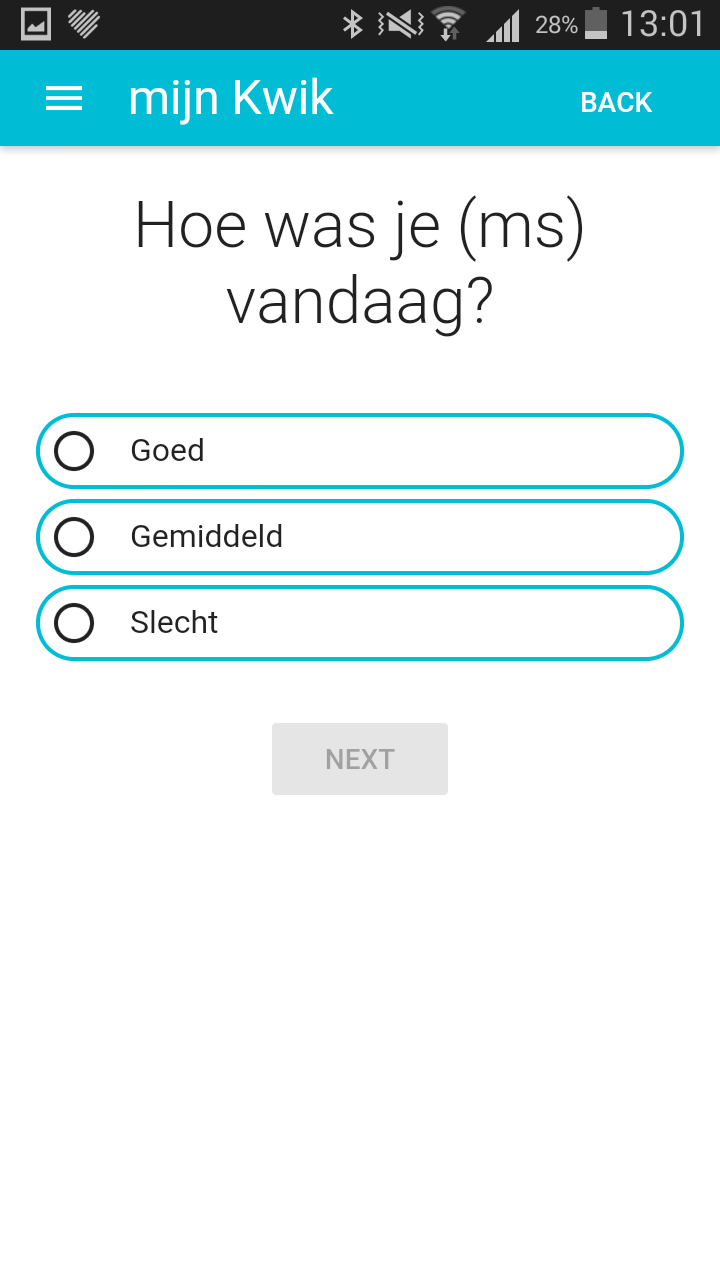
\includegraphics[scale=0.17]{DayIndicator}}
	\hspace{2cm}
	\subfloat[Question about your mood. The slider changes the happiness of the smiley, which represents your feeling today.]{\label{fig:app:mood}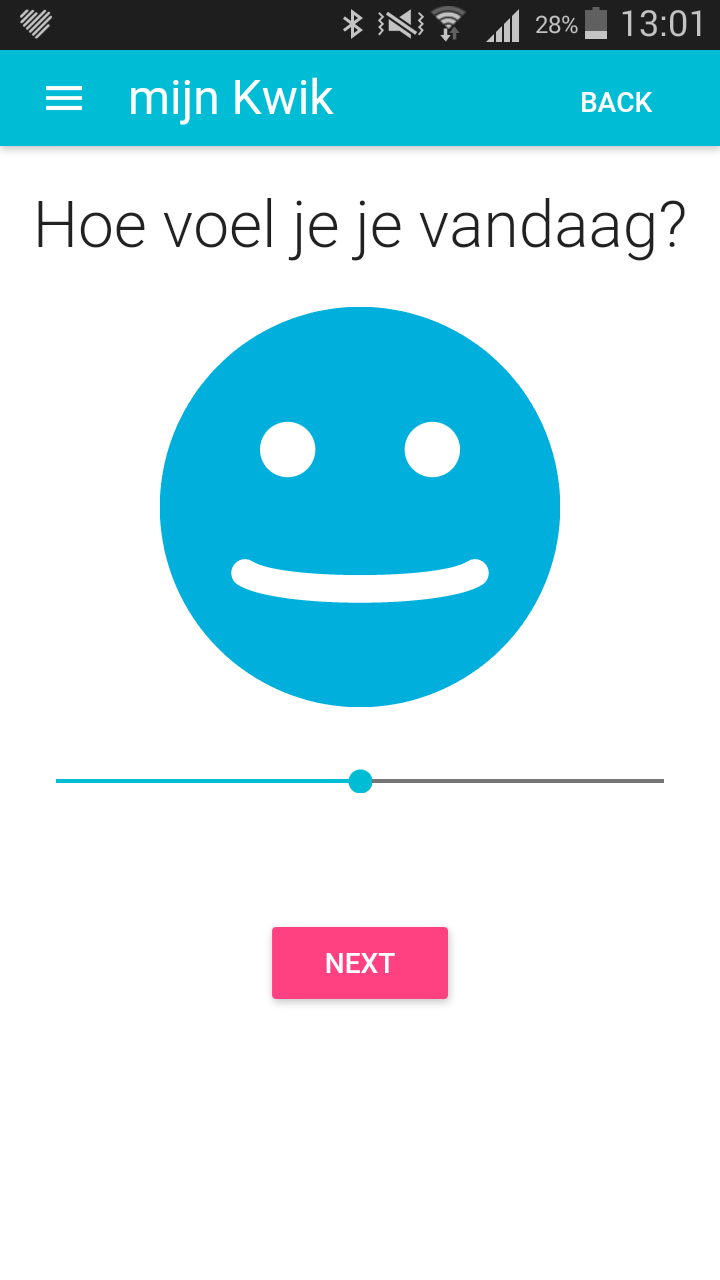
\includegraphics[scale=0.17]{MoodIndicator}}
	\vfill
	\subfloat[The walking test.]{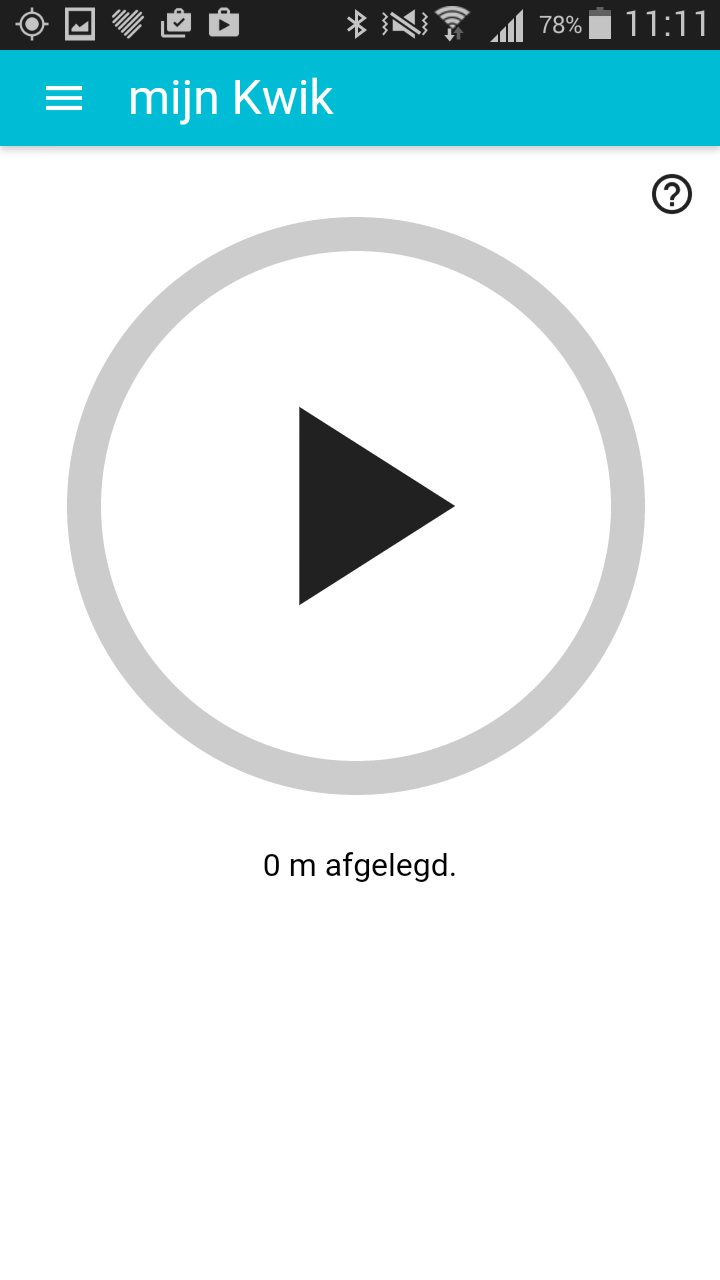
\includegraphics[scale=0.17]{WalkingTest}}
	\hspace{2cm}	
	\subfloat[For the variables \textit{energy}, \textit{mood}, \textit{stress}, \textit{memory}, \textit{concentration} and (not visible in the image) \textit{pain}, give an indication of the current value during this day using the corresponding sliders. ]{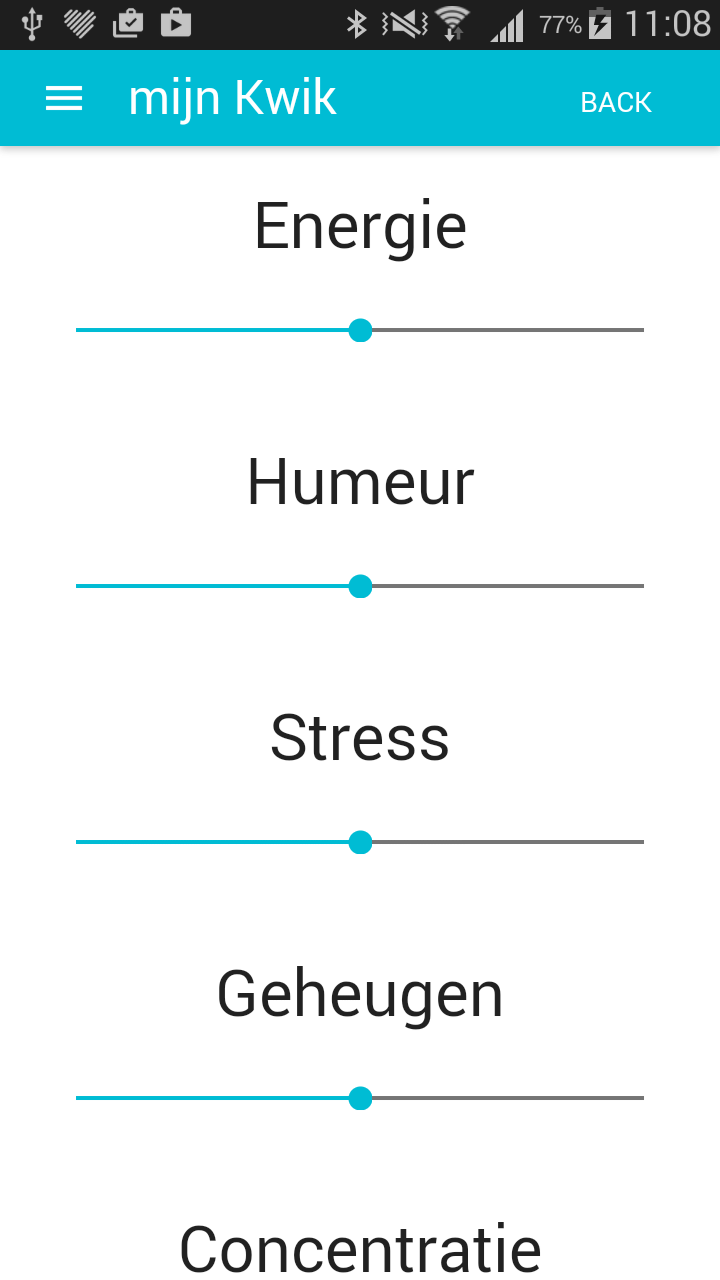
\includegraphics[scale=0.17]{VariablesIndicator}}
	
	\caption{Questions that must be answered and tasks that must be performed  each day in the questionnaire app.}
	\label{fig:app}
\end{figure}
%
All of this data is gathered with the intention to predict good and bad days.
This study will be used to get more insight into the following aspects:
%
\begin{itemize}
	\item Stability of the application;
	\item Ease of use of the wearables and app for MS patients; 
	\item Problems with wearables during the experiment.
\end{itemize}
\parshape=0
%	   if a list has to be included in a paragraph starting with
%      a `lettrine', it is necessary to add the command |\parshape=0|
%      just after the end of the list (starting a new paragraph 
%      just before or just after the list works too)
%
We explained our plans at a meeting for MS patients organized by Orikami.
From all the people that attended the meeting, five patients volunteered to participate in the study.
A second meeting was organized to explain all the necessary details to the participants.
Each of the participants were given one of the following devices:
%
\begin{itemize}
	\item Basis Peak;
	\item Fitbit Charge HR;
	\item Microsoft Wristband 2.
\end{itemize}
\parshape=0
%
With our help, the participants were helped setting up the device and installing the corresponding mobile app on their phones.
Also an user agreement along with a privacy contract were handed out.
The latter had to be signed by each of the participants.
In this privacy contract, it is also stated that all of the gathered data will only be used for research purposes.

\section{Data storage} \label{section: Data storage}
Each of the activity trackers that are handed out to our participants will be linked to the Philips's ``Connect to Healthy''.
Through this service, the captured data will be synced to a database that can be used to access all of the data from the participants.
The data is stored in two databases, one containing the users, the measurement types and the actual measurements from the activity trackers. 
The other database contains the observations done through questions and the types of questions in the questionnaires.
% !TeX spellcheck = en_US
% !TeX root = ../BachelorThesis.tex

\chapter{Analysis of Selected Biomarkers}\label{chapter: Analysis of Selected Biomarkers}
\lettrine[lhang = 0.4, findent=-60pt, lines=7]{\textbf{
		\initfamily \fontsize{40mm}{40mm} \selectfont I
		\normalfont}}{n}
\Cref{section:Selecting Relevant Biomarkers}, we selected three relevant biomarkers: 2MWT, resting heart rate and sleep duration.
In this chapter, we take a closer look at these selected biomarkers.
For each of these selected biomarkers, we look at the corresponding data and combine this data with the questionnaire data for day ratings to see how useful the biomarker can be in predicting good and bad days.
In particular, we want to relate the selected biomarkers to the `How was your MS today?' question in the `Mijn Kwik' application used by the participants.
This specific question can be answered with `good' (goed), `average' (gemiddeld) or `bad' (slecht).
We will be looking at consecutive days, and how these biomarkers possibly play a role in the quality of upcoming days.
Despite the limited dataset (consisting of data gathered over a period of a couple of weeks), we try to get a better understanding of these biomarkers and how they possibly relate to good and bad days.
As noted before, we will be looking at the data of five participants, each of which is identifiable by a unique identity. 
For the patient that was wearing the Microsoft Band 2, the code to integrate the device's data with our database was not finished while writing this thesis.
Therefore, the data from this participant was not used in any of the analyses of the biomarkers.

% !TeX spellcheck = en_US
% !TeX root = ../BachelorThesis.tex

\section{2MWT} \label{section: 2MWT}
We want to investigate if the distance walked during the experiments of the 2MWT could say anything about the quality of the next day. 
Before we can actually use the results of the 2MWT, we must research how accurate and reliable the GPS on mobile phones is.
In Android, there is a method that can give us the accuracy of the retrieved location in meters \cite{androidaccuracy}.
However, this accuracy is only concerned with horizontal accuracy.
Bearing, velocity or altitude are not included.
The GPS is operational under all weather conditions\cite{bar2009geodetic} .
Weather conditions do not influence the accuracy of the position \cite{gpsweather}.
Obstructions like roofs and walls do block GPS signals.
The app should notify the user when the estimated error becomes too big.

Because the earth is not flat, there are actually no straight lines between two GPS coordinates.
To address this problem, there exist several algorithms to calculate the distance between two GPS coordinates.
%
\begin{itemize}
	\item The great-circle distance \cite{weisstein2002great} assumes that the earth is a sphere and uses the spherical law of cosines formula.
	
	\item The haversine formula can also be used to give great-circle distances between two GPS coordinates.
	This formula is better for small distances, because the formula is not too sensitive for a change of input.
	
	\item Methods based on the great-circle distance are less accurate than Vincenty's formula, which assumes that the earth is an oblate spheroid.
	This formula can be accurate up to the millimeter.
\end{itemize}
%
The error in the great-circle distance can be up to 0.5\%, which will result in an error of several centimeters in this case. 
Because the impact of this error is so low, we decided to use the great-circle distance instead.

To get more insight into the accuracy of the measured distance walked, two experiments were designed to test the inter device reliability and accuracy of calculated distance walked in the 2MWT using the `Mijn Kwik' app.
This is the same app that is used by the participants in our study.

\subsection{Experiment 1}

\subsubsection{Method}
In this experiment, we used the straight 100 meters on an all-weather running track as a comparison. The GPS coordinates, used for calculating the total distance walked, are registered at specific time intervals.
These intervals depend on the GPS signal and the used chipset. 
In this case, the time between the registration of consecutive GPS signals was between 4000 and 6000 milliseconds.
To calculate the distance walked, we first used linear interpolation to create a roughly smoothed line through the GPS coordinates.
Afterwards, a Savgol (Savitzky-Golay) filter \cite{press1990savitzky} was used to smooth this raw line. 
The coordinates returned by this Savgol filter where then used used to calculate the distance walked using the great-circle distance.

\subsubsection{Results and Conclusion}
%
\begin{table}
	\centering
	\begingroup
	\fontsize{10pt}{10pt}\selectfont
	\begin{tabular}{@{}lll@{}}
		\toprule
		\textbf{Device} & \textbf{OS}  & \textbf{GPS support} \\ \midrule
		Samsung Galaxy S3 Neo GT-I9301I (1) & 4.4.2 & A-GPS, GLONASS \\
		LG Leon (H320) & 5.0.1 & A-GPS\\
		Samsung Galaxy S3 Neo GT-I9301I (2) & 4.4.2 & A-GPS, GLONASS\\ \bottomrule
	\end{tabular}
	\captionof{table}{Devices used in the experiment.}
	\label{2MWT: exp1 specs}
	\endgroup
\end{table}
%
\begin{table}
	\centering
	\begingroup
		\fontsize{6pt}{7pt}\selectfont
		\begin{tabular}{@{}llllllllll@{}}
			\toprule
			 &  \multicolumn{5}{c}{\textbf{Attempts}}  &  \\ 
			\cline{2-6}
			\textbf{Device}&	\textbf{\#1} & \textbf{\#2} & \textbf{\#3} & \textbf{\#4} & \textbf{\#5} & \textbf{Avg. Error} & \bm{$\tilde{x}$} &  \bm{$\mu$} & \bm{$\sigma$} \\
			\midrule
			Samsung Galaxy S3 Neo GT-I9301I (1) & 140m & 89m & 104m & 95m & 107m & 13.4\% & 104m & 107m & 17.7m\\
			LG Leon (H320) & 96m & 100m & 85m & 91m & 33m & 19\% & 91m & 81m & 24.52m \\
			Samsung Galaxy S3 Neo GT-I9301I (2) & 124m & 127m & 110m & 273m & 155m  & 57.8\% & 127m & 157.8m & 59.42m\\ \bottomrule
		\end{tabular}
		\captionof{table}{Calculated distance walking during each of the attemps.
				For each attempt the median ($\tilde{x}$) and the mean ($\mu$) along with the standard deviation ($\sigma$) are shown.}
		\label{table:walktestresults}
	\endgroup
\end{table}
%
The results of the experiment are shown in \Cref{table:walktestresults}. The specification for each of the phones used in the experiment are shown in \Cref{2MWT: exp1 specs}.
During the experiment, one phone was not able to save the GPS coordinates.
For the results from this phone, no smoothing was applied.
It is unknown why this phone was not able to save these coordinates.
Before using the method that gave us the results shown in \Cref{table:walktestresults} (this method will be discussed later), we used some other methods as well.
As mentioned before, GPS coordinates are given an accuracy value.
Because some GPS coordinates can have an accuracy that is too low, at first we decided to use a threshold value of 50 meters. 
This means that all of the coordinates with an accuracy higher than 50 meter will be filtered. 
Along with this method, we applied the calculation of the walking speed between two consecutive GPS coordinates. 
If this walking speed was higher than 3.0 meters per second, the latter point would not be accepted as a valid one.
The code can be seen in \Cref{walk test code snippet}.

The previous mentioned techniques worked well for some GPS tracks, but failed in others.
Therefore, we decided to test outlier detection using a robust covariance estimator.
Scikit-learn \cite{pedregosa2011scikit} provides an object called Elliptic Envelope.
This object can be used to fit an ellipse to the central data points, ignoring points outside the center.
This gave us better results (\Cref{GPS Plots Straight Line}), although in some cases the quality of the GPS track was too bad to make any prediction at all (\Cref{fig:Terrible GPS Coordinates 1} and \Cref{fig:Terrible GPS Coordinates 2}). As we can see in \Cref{table:walktestresults}, the average error for each of the devices is high.
Most of the readings are not accurate, and there are some extreme cases really differ from the actual distance walked.
Inaccurate GPS signals were influencing our results.
This was easily determined by looking at the unfiltered GPS coordinates.
Even when standing still, the indicated distance walked would increase with tens of meters.
In some extreme cases, this distance would increase with 50 meters during a couple of steps.
The code that was used in the end can be seen in \Cref{GPS Smoothing Code Straight Line}. The plots for the GPS tracks can be seen in \Cref{GPS Plots Straight Line}. \\\\
From this experiment we can conclude that the accuracy and validity of GPS used by phones is something that might require some more investigation.
Even with the two phones of the same model, the average error differs greatly.
This is strange, because in each attempt, all phones were used at once to register the GPS coordinates which were eventually used to calculate the total distance walked.
Because this experiment was only done with a couple of smartphones, these findings are not very representative.

While using the Elliptic Envelope for fitting an ellipse to central data points worked fine when walking in a straight line, it does not work when an arbitrary route is walked which can also have other shapes than a straight line. 
When this is the case, other methods like One-class SVM \cite{oneclasssvm} or clustering algorithms must be used.

\subsection{Experiment 2} \label{Experiment 2}
\subsubsection{Method}
As mentioned in the discussion of Experiment 1, the method applied for detecting outliers in that experiment was not suitable for non-straight tracks. 
Therefore, we decided to use a clustering algorithm to detect the outliers in these kind of GPS tracks.
We choose to use the DBSCAN clustering algorithm.
Density-based spatial clustering of applications with noise (DBSCAN) is a clustering algorithm based on density.
Points that are closely packed together are grouped into clusters.
Points that reside in regions with a low density are marked as outliers.
Both of these classifications are based on the amount of and distance between neighbors.
DBSCAN does not require specification of the number of clusters in the data beforehand.
Another nice property of DBSCAN is that it has a notion of noise, which makes it robust to outliers.
This makes it an excellent algorithm for doing the task of finding clusters in GPS data.
For all the points in the clusters found with DBSCAN, the distance of the GPS coordinates were calculated and added.
Notice that we do not calculate the distance within each cluster separately.
We also calculate the distance between two consecutive points if both points were classified in different clusters.

The track we used in this experiment had a total distance of 115 meters and was circular shaped.
For the calculation of the total distance walked, the same smoothing methods (linear interpolation and Savgol filter) were applied.
As in Experiment 1, the same method for calculating the distance between two GPS-points (great-circle distance) was used.
In this experiment, only one phone was used. 

\subsubsection{Results and Conclusion}
The results for this experiment can be seen in \Cref{table:walktestresults circular}. 
%
\begin{table}
	\centering
	\begingroup
		\fontsize{6pt}{7pt}\selectfont
		\begin{tabular}{@{}llllllllll@{}}
			\toprule
			 &  \multicolumn{5}{c}{\textbf{Attempts}}  &  \\ 
			\cline{2-6}
			\textbf{Device}&	\textbf{\#1} & \textbf{\#2} & \textbf{\#3} & \textbf{\#4} & \textbf{\#5} & \textbf{Avg. Error} & \bm{$\tilde{x}$} &  \bm{$\mu$} & \bm{$\sigma$} \\
			\midrule
			Samsung Galaxy S3 Neo GT-I9301I & 38m & 41m & 133m & 111m & 112m  & 30.6\% & 111m & 87m  & 39.6m \\ \bottomrule
		\end{tabular}
		\captionof{table}{Calculated distance walked during each of the attemps.}
		\label{table:walktestresults circular}
	\endgroup
\end{table}
%
If we plot our GPS coordinates (\Cref{fig:walktestresults example}), we notice that the shape of a ellipse/circle is hardly visible.
Sometimes the coordinates just show a straight line, like some internal system was used to predict future GPS coordinates when the quality decreased or when the signal was lost.
The clustering algorithm (DBSCAN) we decided to use for detecting outliers is working fine for non-straight GPS tracks. 
The major problem is that some GPS measurements are not accurate. If this is the case, this will impact the accuracy of the calculation of the total distance walked.
Because we do not know beforehand what the shape of a GPS track, belonging to one of our participants, is, we will also be using DBSCAN for the analysis of all of the experiments done by our participants.
%
\begin{figure}
	\centering
	\subfloat[]{\includegraphics[scale=0.5]{{Measurement Track}}
	\label{fig: 2MWT attempt}
	}
	\hspace{0.5cm}
	\subfloat[]{\includegraphics[scale=0.319]{{Original Track}}
	\label{fig: 2MWT original}
	}
	\captionof{figure}{Plot of the GPS measurements of one 2MWT attempt (\Cref{fig: 2MWT attempt}) compared to the original walked track (\Cref{fig: 2MWT original}).}
	\label{fig:walktestresults example}
\end{figure}
%

\subsection{General Discussion Experiments}
For both Experiment 1 and Experiment 2, we decided to use linear interpolation and a Savgol filter to smooth our data.
However, there exist a number of other techniques that could be useful as well.
In \cite{jun2005smoothing}, various smoothing techniques were applied to vehicle GPS.
The performance of these algorithms were evaluated on minimizing the impact of random GPS errors in the estimation of speed, acceleration and distance.
The algorithms were least square spline approximation, kernel based smoothing and a modified version of the Kalman filter.
From all these algorithms, the latter was found the most accurate in distance estimation compared to the on-board monitor.
Kalman filters \cite{levy1997kalman} are also frequently used to smooth GPS data. 
We will not go into more details of this algorithm, because the math behind this filter is quite extensive.
However, there seems to be confusion about post processing of GPS data in mobile phones.
Some experts claim that current GPS chips extensively filter the GPS data, while others refute this statement.
If post processing is done in the chips of mobile phones, we would need a second sensor, for example a velocity sensor, to actually improve the data using a Kalman filter.
Kalman filtering is suitable when the input data are noisy. 
If it is used on GPS data with a small sample rate, the track will be much smoother.
However, this will result in a loss of precision. 
Very noisy points will be removed, so that the distance between some GPS points will increase, resulting in a small error in the estimation of the total distance walked.

\subsection{Analysis}
After the experiments into the results from the 2MWT, we take a look at the data from our participants so far.
For the analysis, we used the same algorithm we applied to the data resulting from Experiment 2 (\Cref{Experiment 2}). This also includes the use of DBSCAN clustering on the GPS coordinates.
Looking at data from our participants, we see huge differences between each of the participants.
Some participants regularly did the walking tests while others did not.
For the latter group, most of them have never done any experiment.
We could make a fast conclusion that not having done any walking test makes it hard to say something about this person.
But not having done a walking test for a couple of days or for a longer period of time could also mean a lot.
If a person is too fatigued to be able to do the walking test, no walking tests results would be there.
Therefore, no walking tests results could reflect a poor physical state.
Of course, it is also possible that participants forgot to perform the instructed task for one or several days.
This makes it more difficult to make claims about their physical capabilities.
For the participants that did the walking test regularly, some experiments consisted of positions that would not produce anything useful using DBSCAN clustering.
Looking at these experiments, we see that in the majority of the cases they contain two or even more duplicate coordinates: the start and the end positions. 
To be classified as a cluster, DBSCAN requires more points.
Due to this lack of points, some experiments could not be used.
In the early stages of the experiment also a bug was found in the app.
This resulted in positions that did not contain any latitude or longitude information and making them useless.
This reduced the number of usable experiments.

To get more insight in all the data, we created plots which are shown in \Cref{fig:Walking Test Visualization}.
Each letter of the plot corresponds with the participants in \Cref{table: Walking Test Analysis}. 
Only for the person that did not do a single walking test (\Cref{table:user5}) no plot is shown.
For both participant \subref{fig:user1} and participant \subref{fig:user2}, some results of the walking tests (200+ meters walked) seem to be inaccurate. 
Given that an average healthy person walks 5 kilometers per hour, it is possible to walk a distance of roughly $5/3.6 \cdot 120 \approx 167$ meters. 
Because MS patients often find it difficult to walk, it is unlikely that such distances would be walked in the performed walking tests.
It is also possible that some people really wanted to challenge themselves and therefore performed really well.
In \cite{nogueira2013factors}, factors for lower walking speed for persons having MS were analyzed.
By using only a track of 10 meters, it was found that 85\% of the patients showed a lower walking speed.
This makes the statement of highly motivated participants less likely.
To validate the hypothesis of inaccurate GPS tracks causing a high distance walked, we would need more participants for comparison.

Before actually looking at the data to inspect the relation between day ratings and measurements, we have to find out how both the distance walked and the day rating are related with each other.
For this we need to use some form of statistical test.
Before actually choosing a statistical test, we need to know what the level of measurement for all of our involved variables is.
For the ratings we have three different categories: `good', `average' and `bad'.
The level of measurement for the variable `day rating' clearly is ordinal.
The level of measurement for the variable `distance walked' is ratio (this also same for the measurements of heart rate and sleep duration).
There are a lot of statistical tests available to research the association between two variables. 
Using \cite{nayak2011choose}, we find that both the Spearman's rank correlation coefficient $\rho$ and the Kendall's rank correlation coefficient $\tau$ are applicable.
The values of Kendall's $\tau$ are usually smaller than the values Spearman's $\rho$. 
Because Spearman's $\rho$ is based on deviations, it is more sensitivity to errors compared to Kendall's $\tau$.
Because it is very likely that our data is contaminated with inaccurate data, we decided to choose Kendall's $\tau$ to investigate the association between the two variables.
Kendall's rank correlation is a correlation coefficient based on the ranks of the data instead on the data itself. 
The results of the application of the algorithm can be seen in \Cref{table:walking test kendall tau}.
In this table, we also see a so called $p$-value.
When the Kendall's rank correlation coefficient is used to determine whether two variables are related or not, the null hypothesis of independence of the two used variables has an expected value of zero.
According to the documentation of the used implementation of Kendall $\tau$ from SciPy, this $p$-value is ``the two-sided $p$-value for a hypothesis test whose null hypothesis is an absence of association'' \cite{kendalltauscipy}.
The two-sided (or two-tailed) $p$-value allows to test the statistical significance in both directions. 
This means that you are testing for the possibility of a relation in both directions.
As we can seen in \Cref{table:walking test kendall tau}, the correlation coefficients for participant \subref{fig:user2} and \subref{fig:user3} are not shown. 
This is because the algorithm for calculating the correlation coefficient returned NaN (Not a Number) for both of the corresponding measurements. 
Because we investigate the relation between the measurement and the rating of the day after, we drop our first rating and our last measurement.
This makes sure that for each measurement, the rating of the next day is used to see if there is a relation between the two of them.
If we have only two measurements and corresponding ratings, the method described above will leave us only with one measurement and one rating.
This is not enough to calculate the Kendall's correlation coefficient. 
Therefore, the entries for these two figures resulted in NaN values.
%
\newpage
\begin{table}[H]
	\centering
	\begin{tabular}{@{}lll@{}}
		\toprule
		\textbf{Participant} & \bm{$\tau$} & \bm{$p$}\\
		\midrule
		\subref{fig:user1} & $0.40$ & $0.414935$ \\
		\subref{fig:user4} & $0.0$ & $1.0$  \\ 
		\bottomrule
	\end{tabular}
	\captionof{table}{Expressing the rank correlation between distance walked and day rating.}
	\label{table:walking test kendall tau}
\end{table}
%
\begin{figure}[H]
	\centering
	\subfloat[]{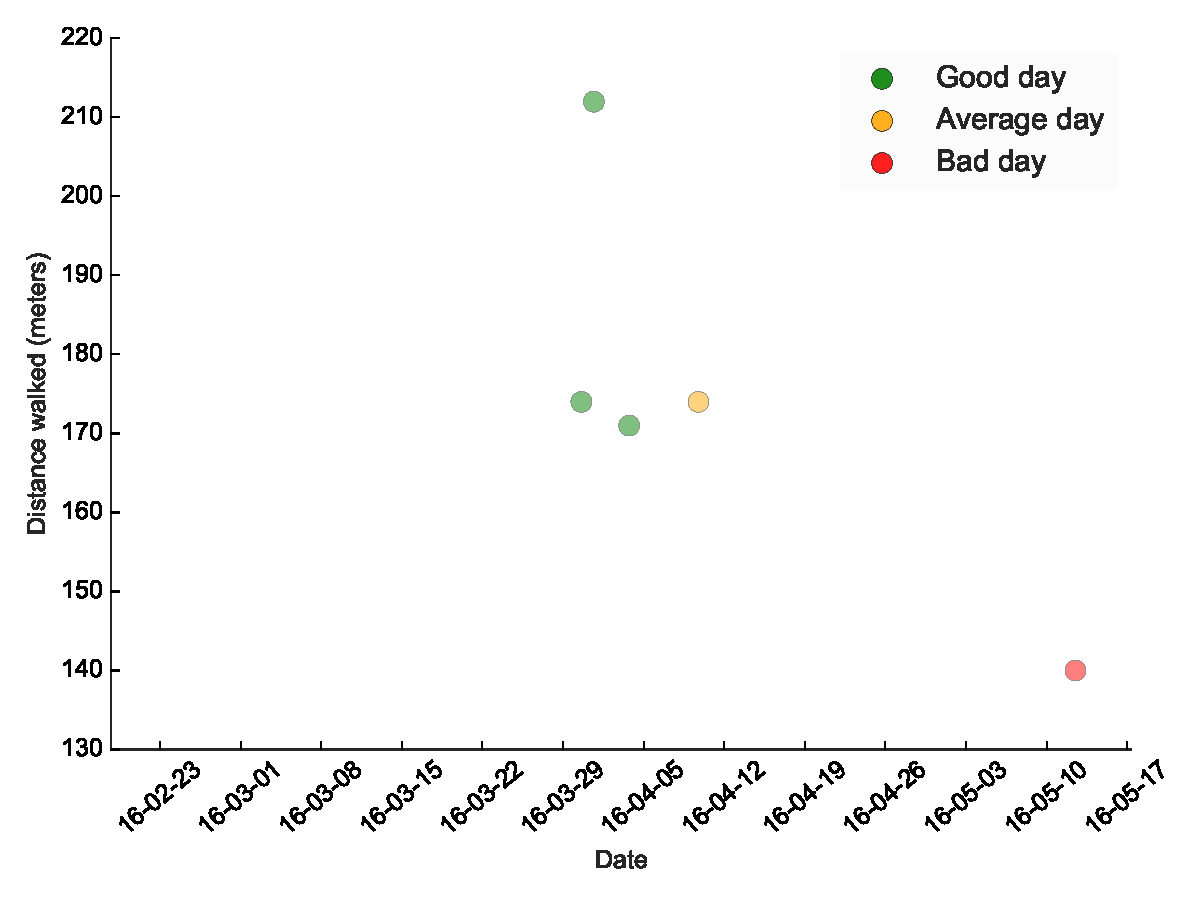
\includegraphics[scale=0.29]{img/walking/2Dy2uFf3aw6jv9r5u}
		\label{fig:user1}
	}
	\hspace{0.5cm}
	\subfloat[]{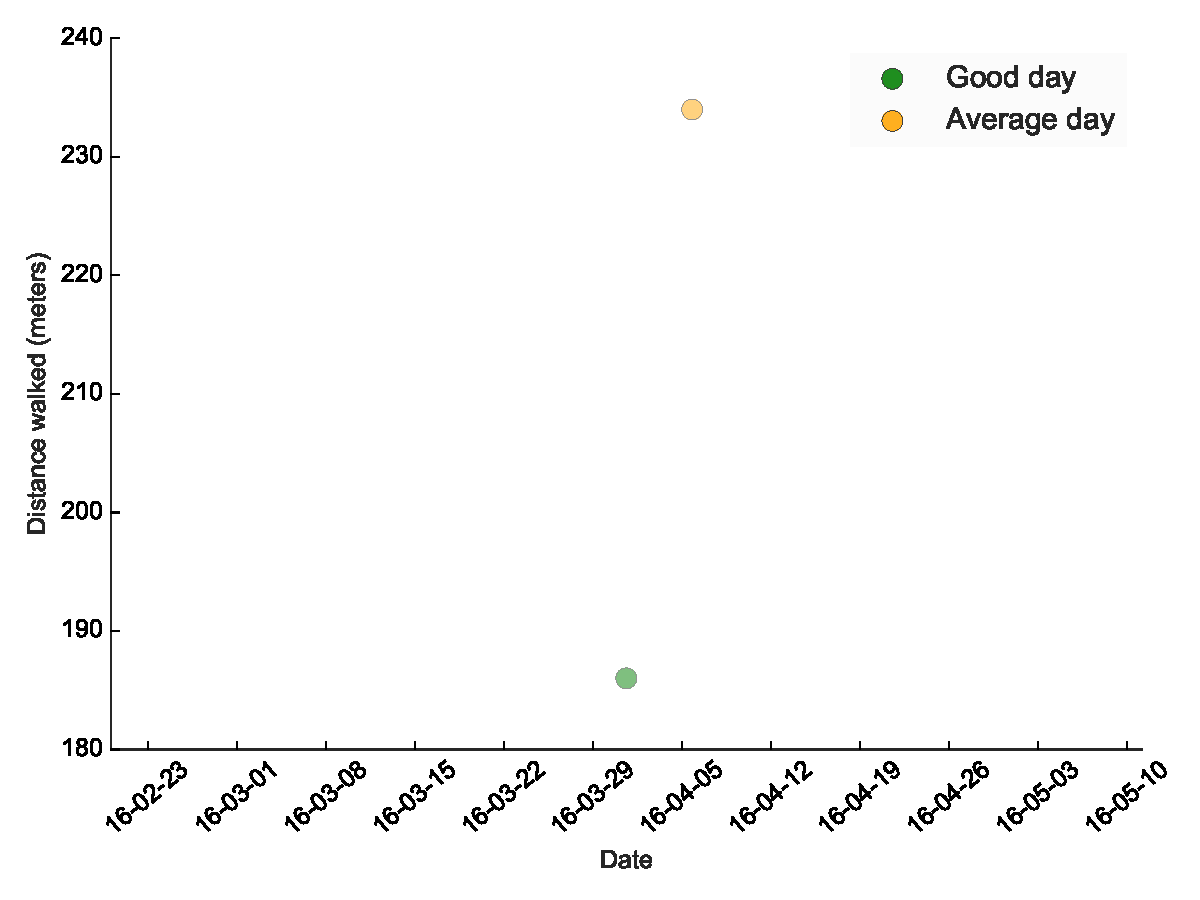
\includegraphics[scale=0.29]{img/walking/dW4YzJQEaidmyhsuY}
		\label{fig:user2}
	}
	\vfill
	\subfloat[]{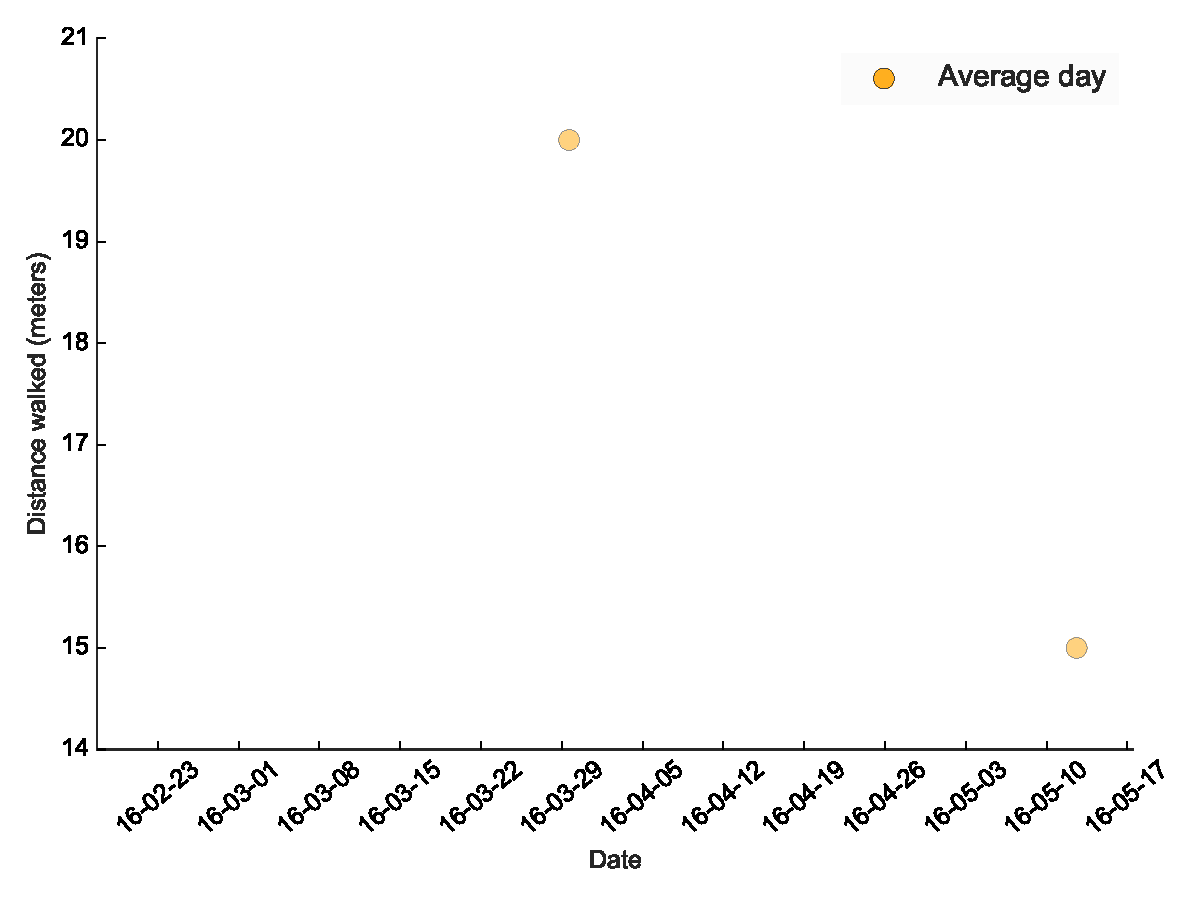
\includegraphics[scale=0.29]{img/walking/gGSWzh5PnqgFdCpq4}
		\label{fig:user3}
	}
	\hspace{0.5cm}
	\subfloat[]{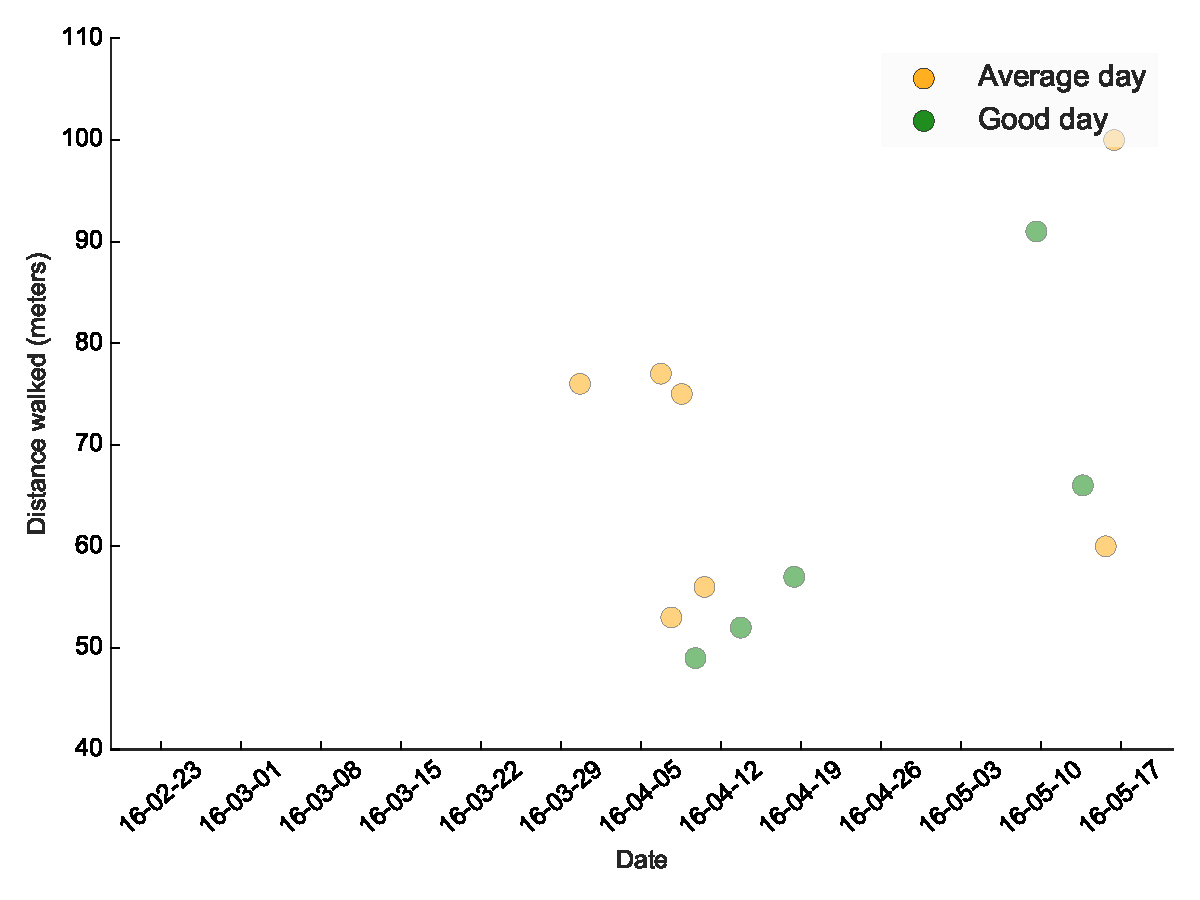
\includegraphics[scale=0.29]{img/walking/oGTtb7DQu4ewMBinx}
		\label{fig:user4}
	}
	\captionof{figure}{Plots of the walking durations of the participants. 
		Only dates that both had a rating and a measurement of distance walked are shown. 
		As can be seen in the legend of each of the figures, each point is colored according to the rating given by the participant for that specific day.}
	\label{fig:Walking Test Visualization}
\end{figure}
\newpage
%
To interpret the rest of the coefficients, we must look at the outcome of the correlation coefficient.
%
\begin{itemize}
	\item A positive correlation coefficient means that the ranks of both the variables are increasing.
	\item A negative correlation coefficient means that if the rank of one variable increases, the rank of the other variable decreases. 
	\item If both variables are independent, a coefficient with a value of zero would be expected.
\end{itemize}
%
For the other participants (\subref{fig:user1} and \subref{fig:user4}), the amount of samples is better.
For all of the coefficients, the corresponding $p$-value is never lower than $0.05$.
Therefore, there is no sign of statistical significance for each of the coefficients.
This lack of statistical significance makes it useless to try to interpret the correlation coefficients.
In the end, it seems like the amount of experiments for most of the participants is just too low to get meaningful results using statistical analysis.
% !TeX spellcheck = en_US
% !TeX root = ../BachelorThesis.tex

\section{Resting Heart Rate}
Every minute, the heart rate of a participant is measured by the activity tracker and eventually stored in the database. 
In \Cref{table: Heartrate Analysis}, we see the heart rates of our participants.
The corresponding plots can be seen in \Cref{fig: heart rates plots}.
As one can notice, not all the dates visible in each of the boxplots in \Cref{fig: heart rates boxplots} are in these plots. 
This is because all participants did not give a rating for some days.
Although we do not know for sure why this is the case, this is probably because they forgot to do so.
We also excluded these days without ratings in each of the tables in \Cref{table: Heartrate Analysis}.
In contrary to our first investigated biomarker (2MWT), we can see that a lot more measurements are present in \Cref{fig: heart rates plots}.
Because each device automatically measures the heart rate, there is no user intervention required which definitely has a positive effect on the amount of data.

If we take a look at the boxplots in \Cref{fig: heart rates boxplots}, we see that the majority of the fliers (outliers) are in the high regions of the boxplots.
In the lower parts, we rarely see fliers.
This observation gave us the insight that the average of the lowest 5\% of the measurements is probably a good and stable estimation of the resting heart rate of the participant for a single day.
Therefore, the plots show the average of the lowest 5\% of the heart rates measurements and not the average of all the measurements for that day.
For each participant, Kendall's $\tau$ correlation coefficient along with the $p$-values can be seen in \Cref{table:resting heart rate kendall tau}.
As we have seen in \Cref{section:Resting Heart Rate}, the resting heart rate for adult lies between 60 and 100 beats, which is also suggested by the figures in \Cref{fig: heart rates plots}.
In \Cref{section:Resting Heart Rate}, we have also seen that a low resting heart rate is more desirable than a high one.
Looking at the plot from participant \subref{fig:heart user2}, we see exactly the opposite of what we would have expected: for most of the lower resting heart rates, the day ratings tend to go worse. 
The day on which the participant had his lowest resting heart rate was rated as `bad'.
For participant \subref{fig:heart user1}, such a relation is not visible as the data seems to be spread randomly.

In \Cref{table:resting heart rate kendall tau}, we see that the correlation coefficient for participant \subref{fig:heart user3} is close to zero.
The coefficients for participants \subref{fig:heart user2} and \subref{fig:heart user4} tend to go negative, suggesting that if the rank of the average of the lowest 5\% of the heart rate measurements decreases, the rank of the rating increases (which we also noticed by ourselves). 
None of the $p$-values is near 0.05.
This indicates that the effect observed in the data is likely, even assuming that the null hypothesis of no effect is true.
For this particular biomarker, the null hypothesis would state that there is no relation between the average of the lowest 5\% of the heart rates and the rating of the day after.
%
\newpage
\begin{table}[H]
	\centering
	\begin{tabular}{@{}lll@{}}
		\toprule
		\textbf{Participant} & \bm{$\tau$} & \bm{$p$}\\
		\midrule
		\subref{fig:heart user1} & $0.128873$ & $0.254708$ \\
		\subref{fig:heart user2} & $-0.176887$ & $0.305310$ \\
		\subref{fig:heart user3} & $0.021340$ & $0.842163$ \\
		\subref{fig:heart user4} & $-0.174944$ & $0.210129$ \\
		\bottomrule
	\end{tabular}
	
	\captionof{table}{Expressing the rank correlation between the average of the lowest 5\% of the heart rate measurements and the day rating.
	}
	\label{table:resting heart rate kendall tau}
\end{table}
%
\begin{figure}[H]
	\centering
	\subfloat[]{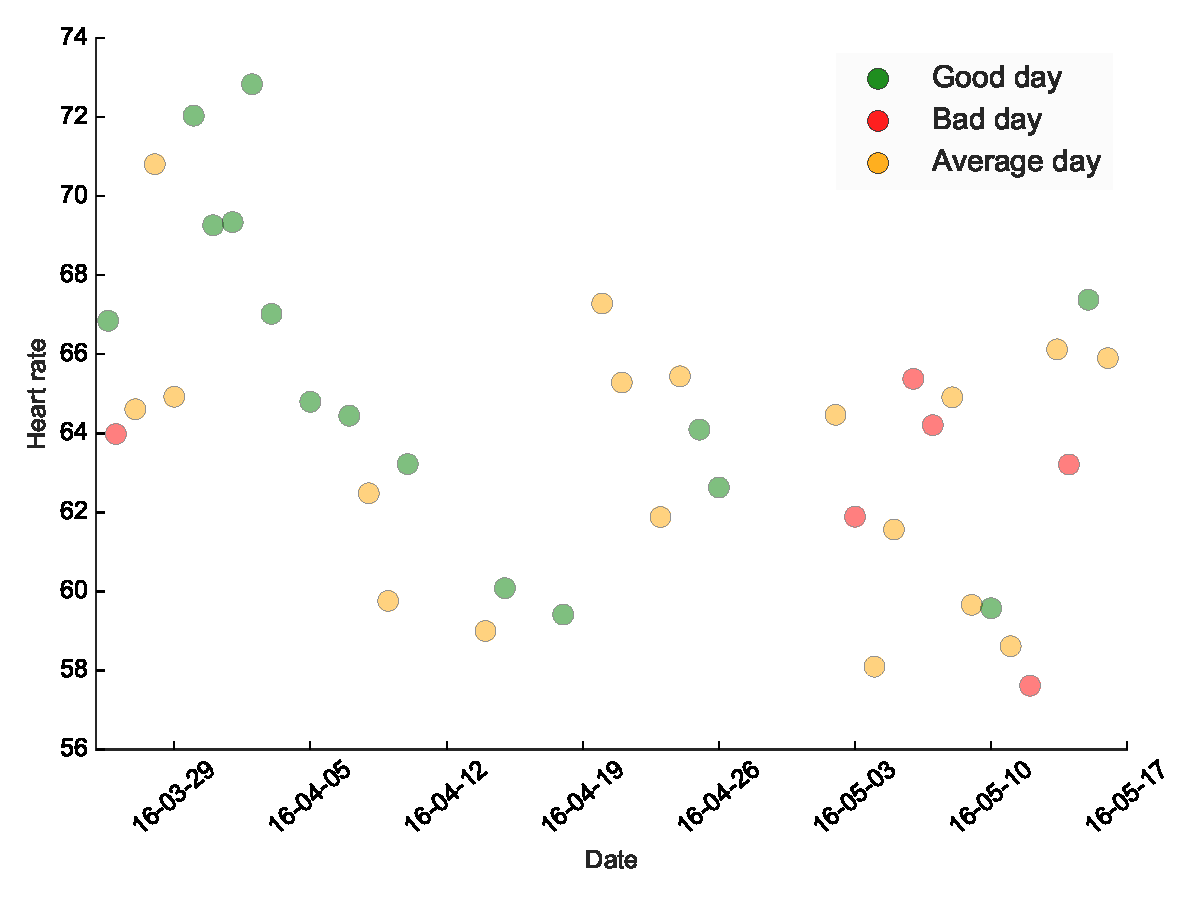
\includegraphics[scale=0.29]{img/heartrate/2Dy2uFf3aw6jv9r5u}
		\label{fig:heart user1}
	}
	\hspace{0.5cm}
	\subfloat[]{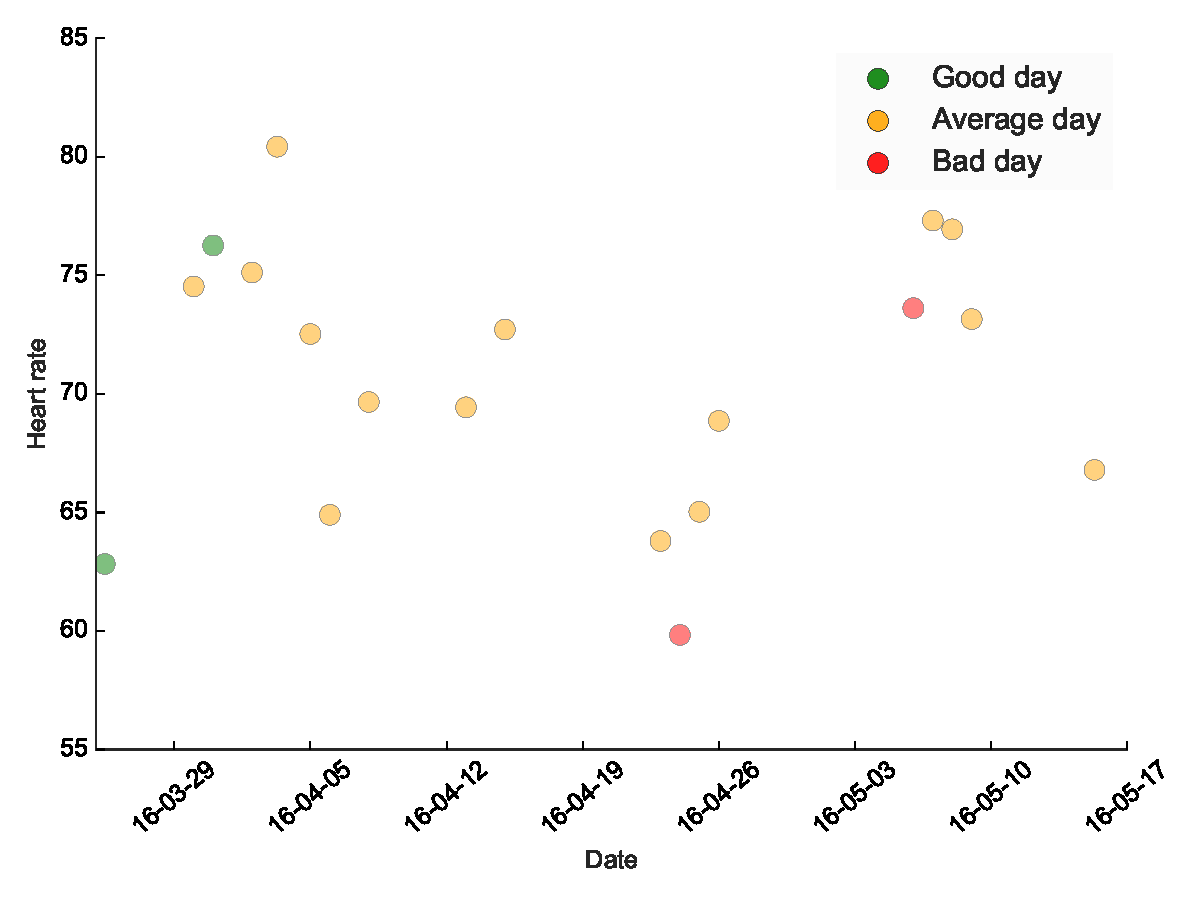
\includegraphics[scale=0.29]{img/heartrate/dW4YzJQEaidmyhsuY}
		\label{fig:heart user2}
	}
	\vfill
	\subfloat[]{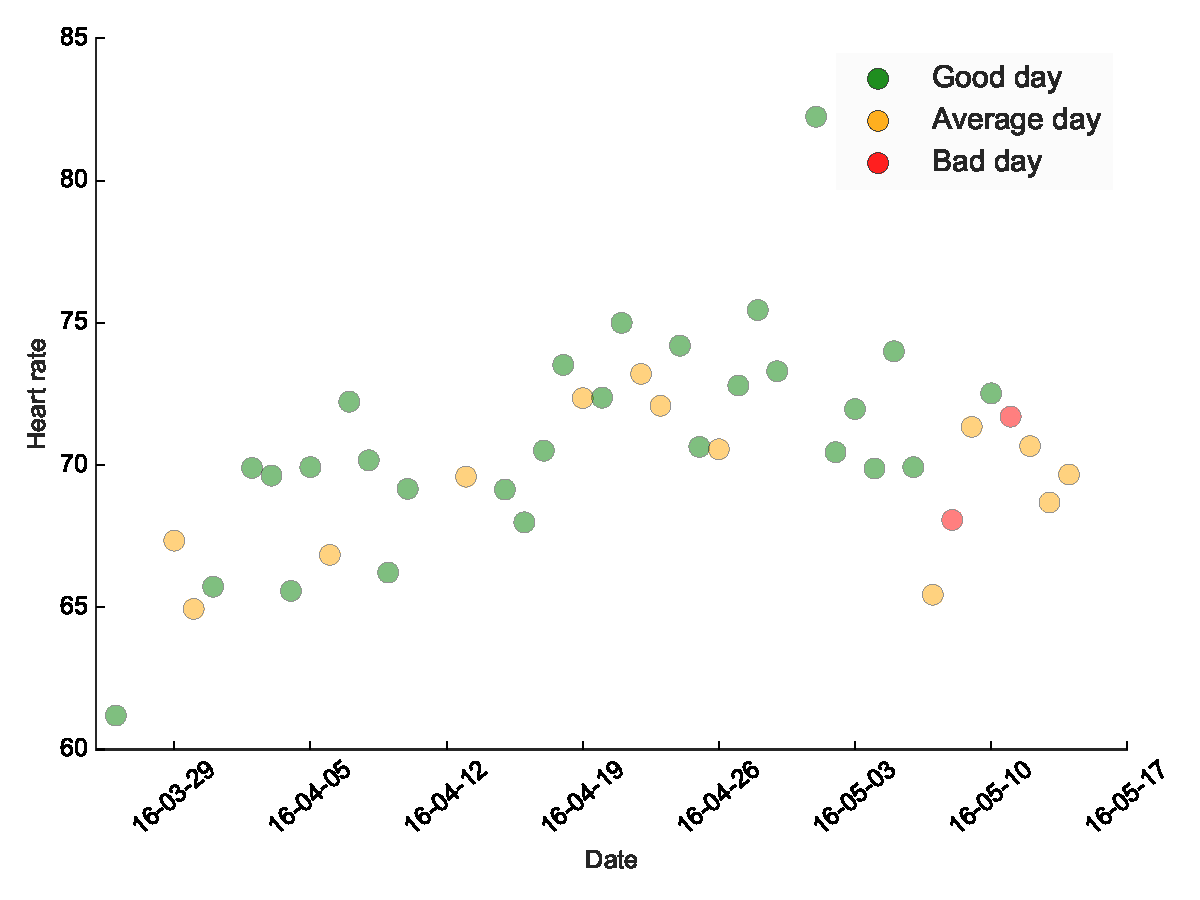
\includegraphics[scale=0.29]{img/heartrate/gGSWzh5PnqgFdCpq4}
		\label{fig:heart user3}
	}
	\hspace{0.5cm}
	\subfloat[]{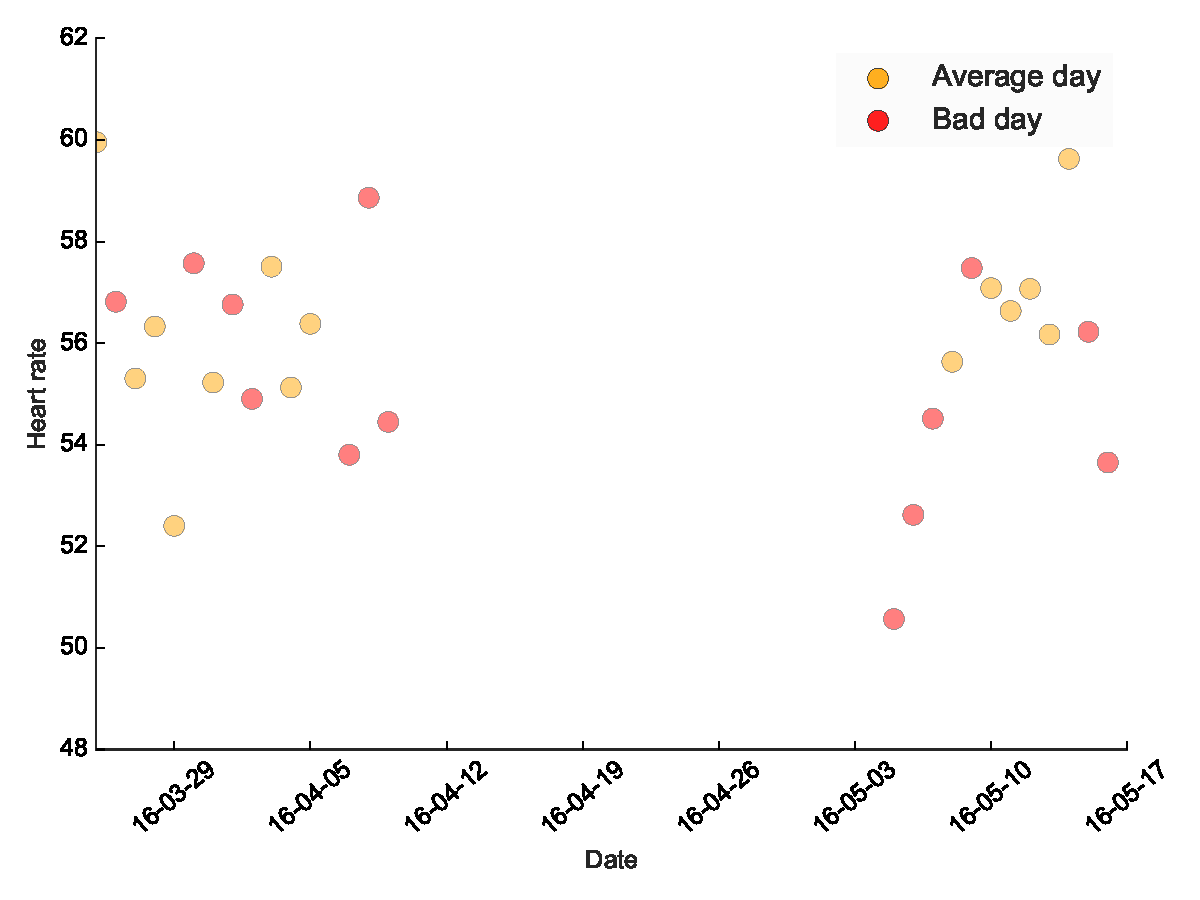
\includegraphics[scale=0.29]{img/heartrate/S2usWtx8WXPe8S88r}
		\label{fig:heart user4}
	}
	\captionof{figure}{Plots of the average from the lowest 5\% of the heart rates measurement of the participants for each day. 
	Only dates that both had a rating and measurements of heart rates are shown. 
	As can be seen in the legend of each of the figures, each point is colored according to the rating given by the participant for that day.}
	\label{fig: heart rates plots}
\end{figure}
\newpage
%
\input{chapters/"Sleep Duration"}

% !TeX spellcheck = en_US
% !TeX root = ../BachelorThesis.tex

\chapter{Conclusion and Discussion}\label{chapter: Conclusion and Discussion}
\lettrine[lhang = 0.4, findent=-60pt, lines=7]{\textbf{
		\initfamily \fontsize{40mm}{40mm} \selectfont I
		\normalfont}}{n}
this thesis, we have looked at relevant biomarkers in the prediction of good and bad days for multiple sclerosis (MS) patients. 
Because activity trackers were used, the validity and reliability was reviewed in \Cref{section: Reliable Data Collection}.
In this section it was found that activity trackers are widely used in the research field and that the measurement of most of the health related variables are an accurate representation of the true values.
In \Cref{section:relevant biomarkers}, we have conducted a literature review for relevant biomarkers. 
This was done by looking at how biomarkers can be measured and how they are currently being used or could be used to get more insight in the health state of (MS) patients.
In \Cref{section: 2MWT}, two experiments were designed and conducted to test the reliability of GPS coordinates that were used to calculate the distance walked in the 2MWT.
In both experiments it was found that the quality of the GPS tracks would differ a lot.
There were tracks that would give a good approximation of the total distance walked but other tracks were of insufficient quality to get a good estimation.
From the result of the final experiment, it was decided that applying clustering on the GPS points belonging to a GPS track would detect the outliers.
These outliers are excluded in the algorithm for calculating the total distance walked.
After reviewing existing usage of biomarkers in \Cref{section:Selecting Relevant Biomarkers}, we chose the following biomarkers for investigating their relation with good and bad day analysis: 2MWT, resting heart rate (RHR) and sleep duration.
For the results of the 2MWT, the final algorithm which makes use of clustering was used to calculate the distance walked in the analysis of the data from the participants.
For each individual biomarker, we investigated its relation with the day rating of the next day by using statistical analysis.
Although we found some relations that confirmed or refuted some of our hypotheses, their was too much diversity to conclude anything.
The restricted dataset and number of participants contributed to this. 
We also found that some data seemed to be missing and that participants were forgetting to rate days using the `Mijn Kwik' app.
Especially data, that required the participant to perform specific tasks in order to become available, was missing.
To minimize the risk of missing data due to participant in future research, most of the measurement should be done automatically if possible.

Although we focused on a small selection of biomarkers to investigate their potential as a biomarker in the prediction of good and bad days for MS patients, we do not exclude the use of others.
As an example, another biomarker was `found' during a hackathon.
In the weekend of 21-22 May 2016, this MS hackathon was organized in Amsterdam, the Netherlands%
\footnote{\url{http://www.mshackathon.nl}}.
In this hackathon, a variety of people worked together to gain new insights into MS for researchers, doctors and patients themselves.
A team from Orikami also participated in this hackathon.
Currently there is not an objective scale to measure fatigue.
People that have to indicate themselves how fatigued they are, seem to have problems with this: they are not able to correctly make an estimation of their current fatigue.
Relatives however are often able to see when people are fatigued, although these people cannot see this by themselves.
In current literature, the relation between eye movement and fatigue has already been investigated \cite{Arief_2009}.
Based on these findings, we came up with the idea to measure fatigue based on recordings from the eye.
By letting the user focus on a screen on which circles appear randomly, we can determine how fast the eye responds on these events.
Using these measurement, we would like to get an objective measurement of the fatigue level from MS patients.
The idea was also appreciated by specialists and MS patients and we even managed to win the 2nd place.
In the future, this new technique should be investigated even more to get a more accurate measurement on fatigue for MS patients.

Because this thesis can be seen as an exploratory study, the lack of any relation between the investigated biomarkers and the day ratings was in line with our expectations.
In upcoming research, investigating the relation between biomarkers and the quality of upcoming days could be done using more sophisticated methods.
This should also include analysis in which multiple biomarkers are considered at the same time.

\bibliographystyle{plain}
\bibliography{bib/Bibliography}

% !TeX spellcheck = en_US
% !TeX root = ../BachelorThesis.tex
\appendix
\numberwithin{figure}{section}
\chapter{Appendix}

\section{GPS Plots Straight Path}
%
\begin{figure}[H]
	\centering
	\subfloat[]{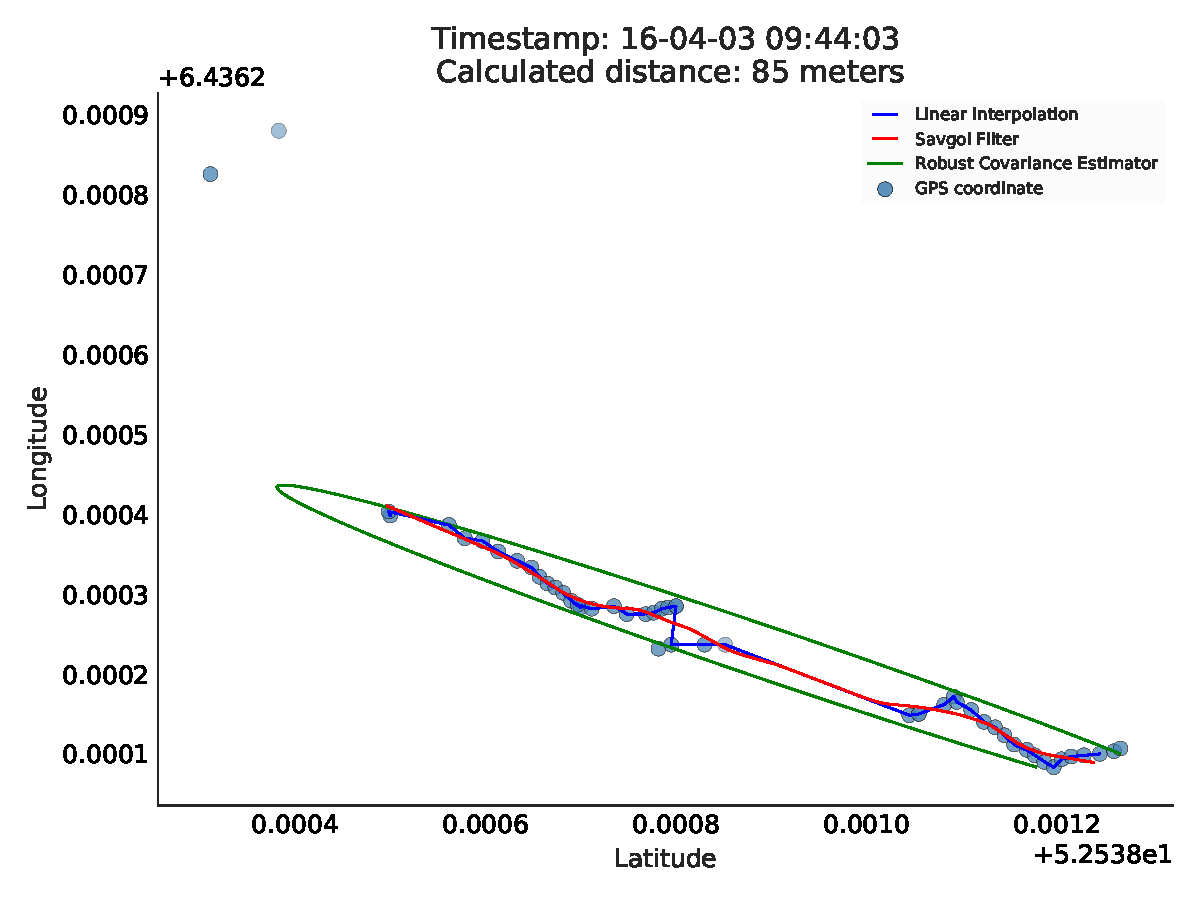
\includegraphics[scale=0.29]{gps/straight/3wAkwQDaLY7gYrhPi}
	}
	\hspace{0.5cm}
	\subfloat[]{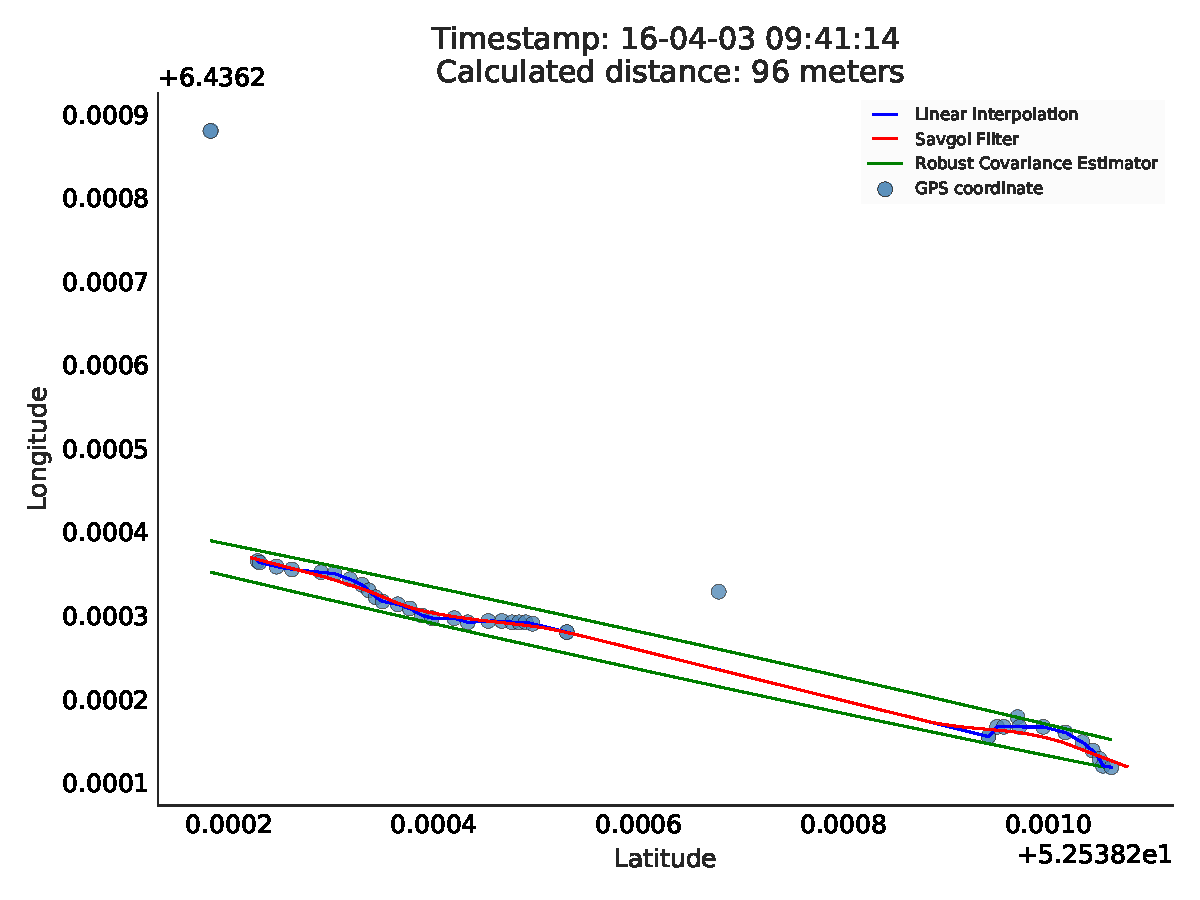
\includegraphics[scale=0.29]{gps/straight/9cuCTXcBBK2J32PoE}
	}
	\vfill
	\subfloat[]{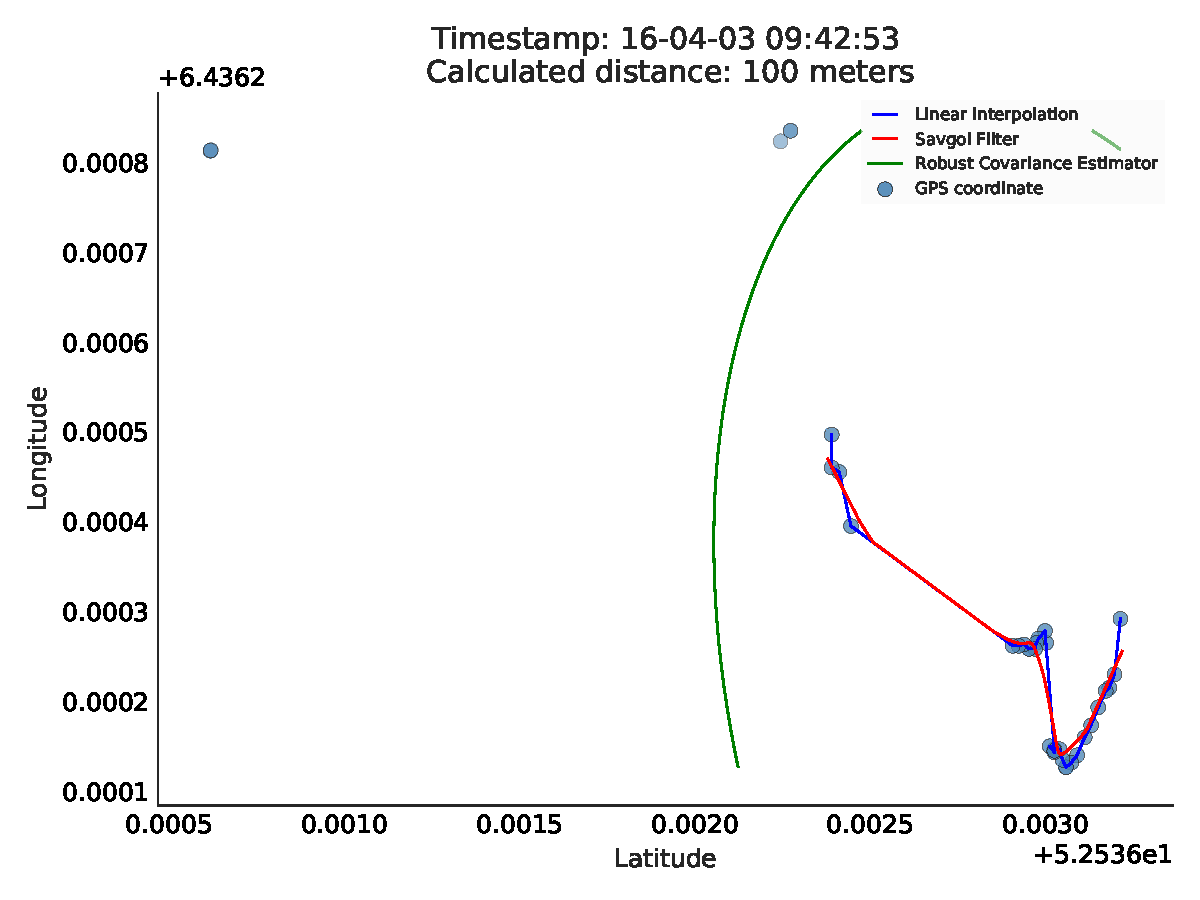
\includegraphics[scale=0.29]{gps/straight/Ba8aoCEfdhz2nxYq9}
	}
	\hspace{0.5cm}
	\subfloat[]{\label{fig:Terrible GPS Coordinates 1}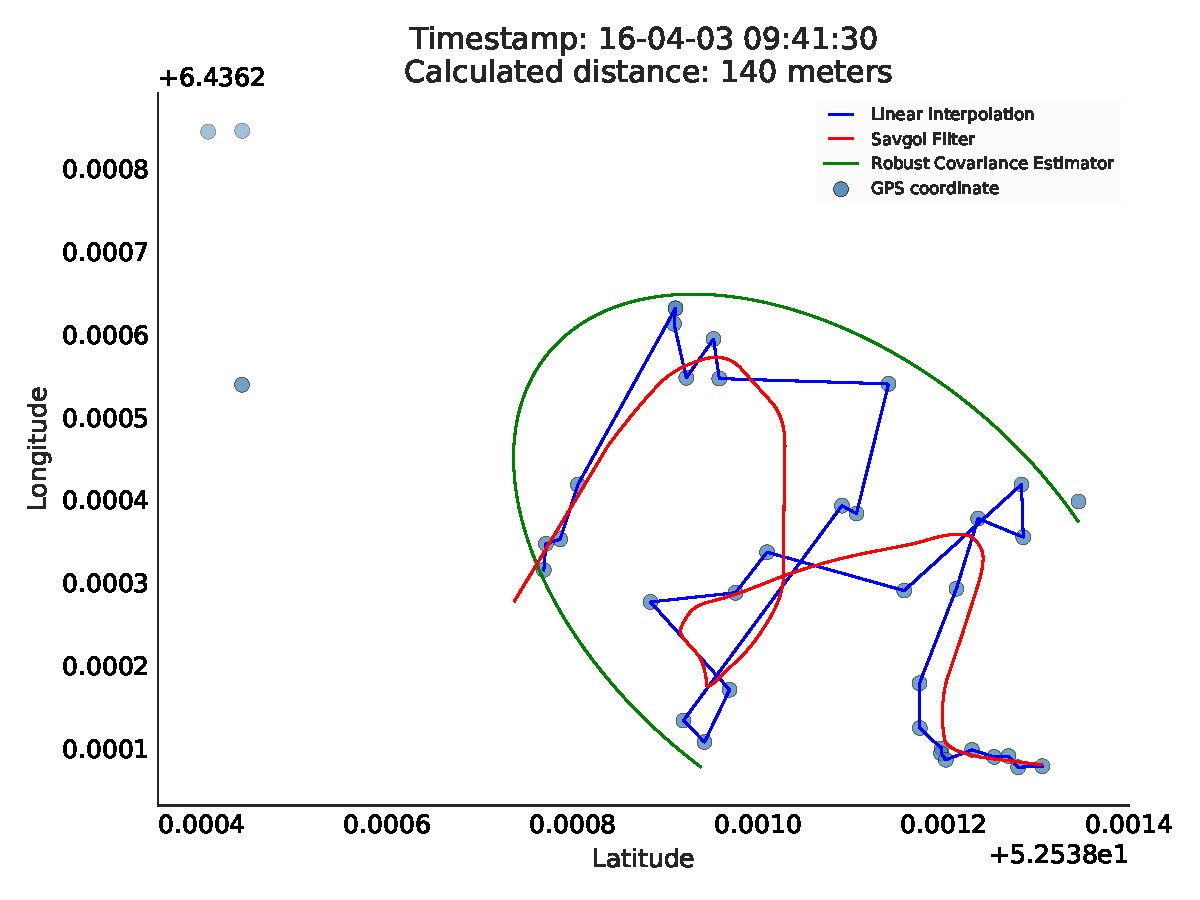
\includegraphics[scale=0.29]{gps/straight/CbpZDcgq8d6BCy5mj}
	}
	\captionof{figure}{Plots of the GPS coordinates of the walking test before and after smoothing. First, outlier detection is done using Elliptic Envelope. Afterwards, inliners are  smoothed in two stages: `Lineair Interpolation' is the first smoothing step and `Savgol Filter' the last.}
	\label{GPS Plots Straight Line}
\end{figure}
%
\begin{figure}[H]
	\ContinuedFloat 
	\centering
	\subfloat[]{\label{fig:Terrible GPS Coordinates 2}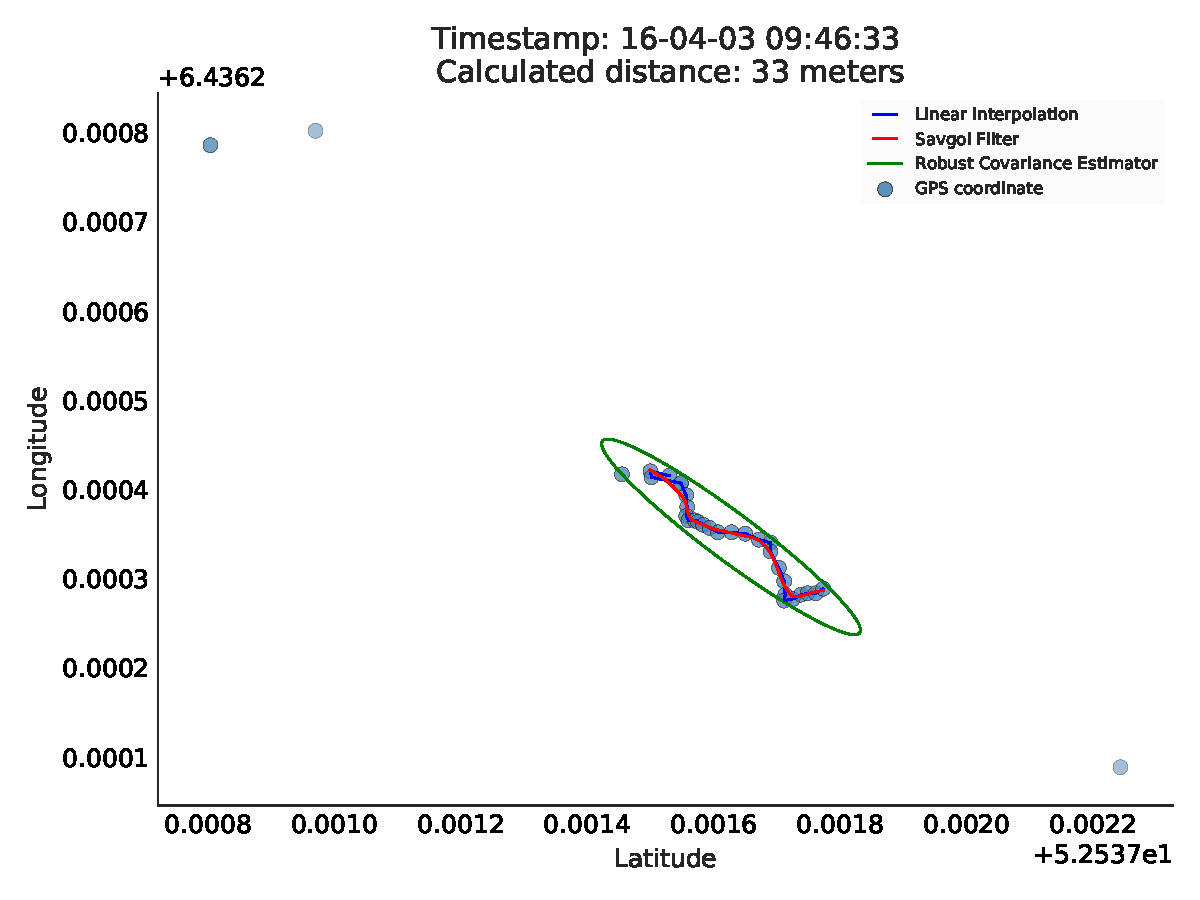
\includegraphics[scale=0.29]{gps/straight/exCkb4K2cCaZHHg4b}
	}
	\hspace{0.5cm}
	\subfloat[]{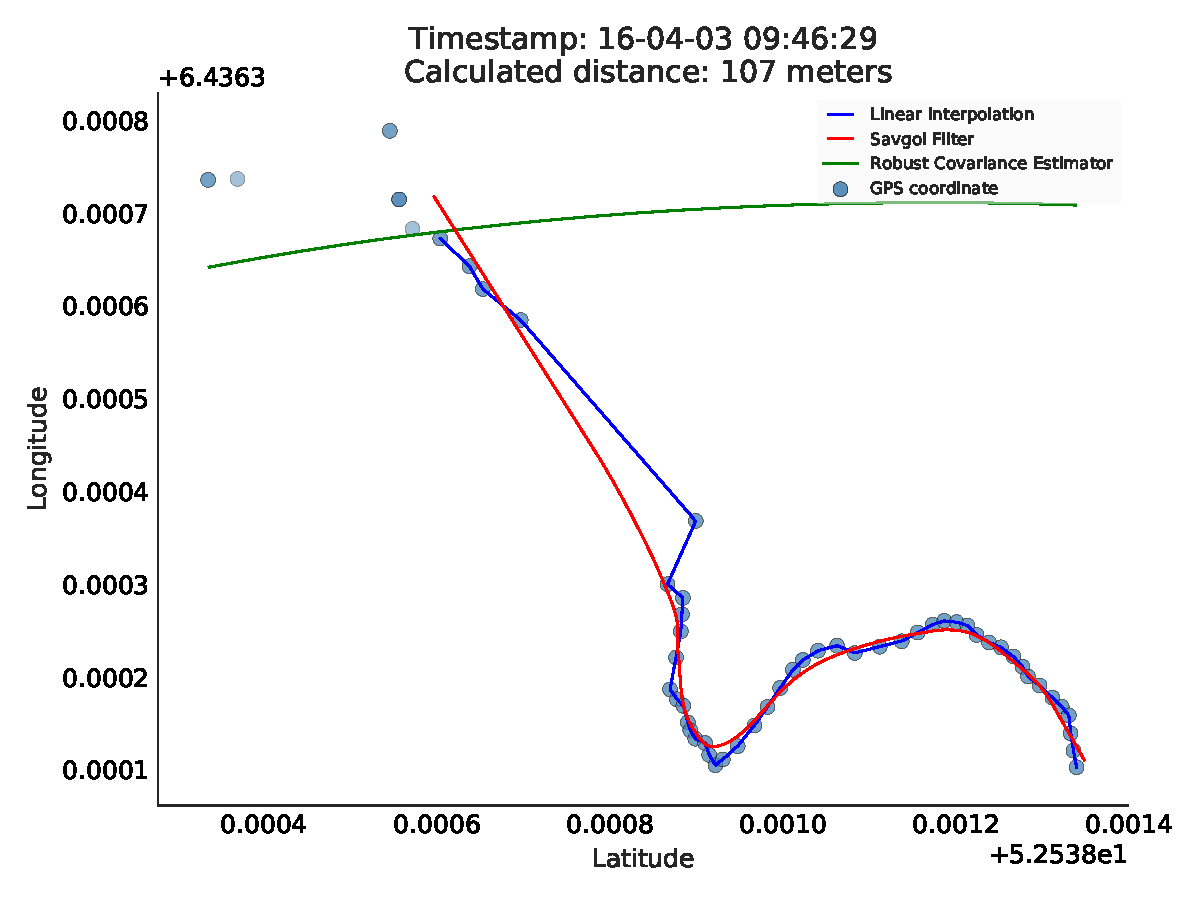
\includegraphics[scale=0.29]{gps/straight/fA2QJHC6iPcAmnu4x}
	}
	\vfill
	\subfloat[]{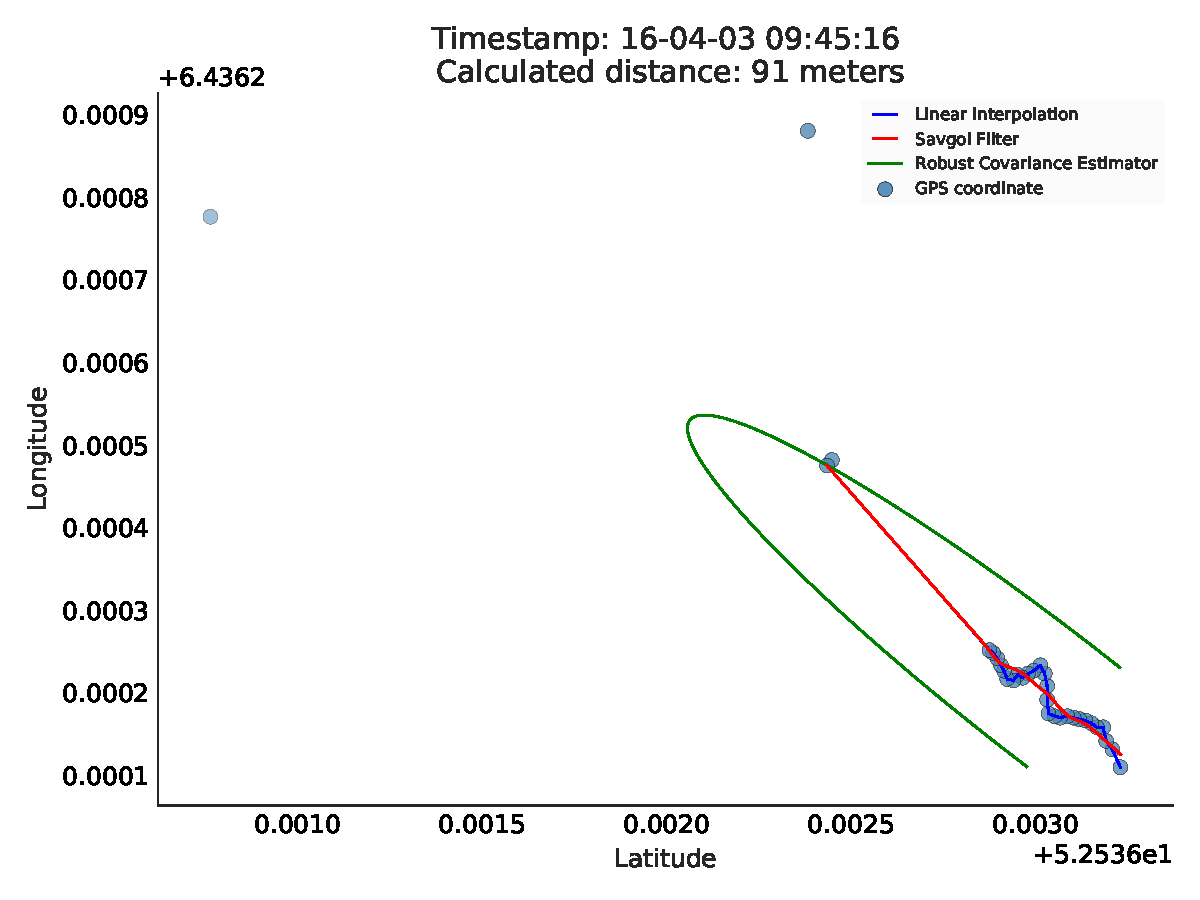
\includegraphics[scale=0.29]{gps/straight/g7zX6A4FnTu4L975N}
	}
	\hspace{0.5cm}
	\subfloat[]{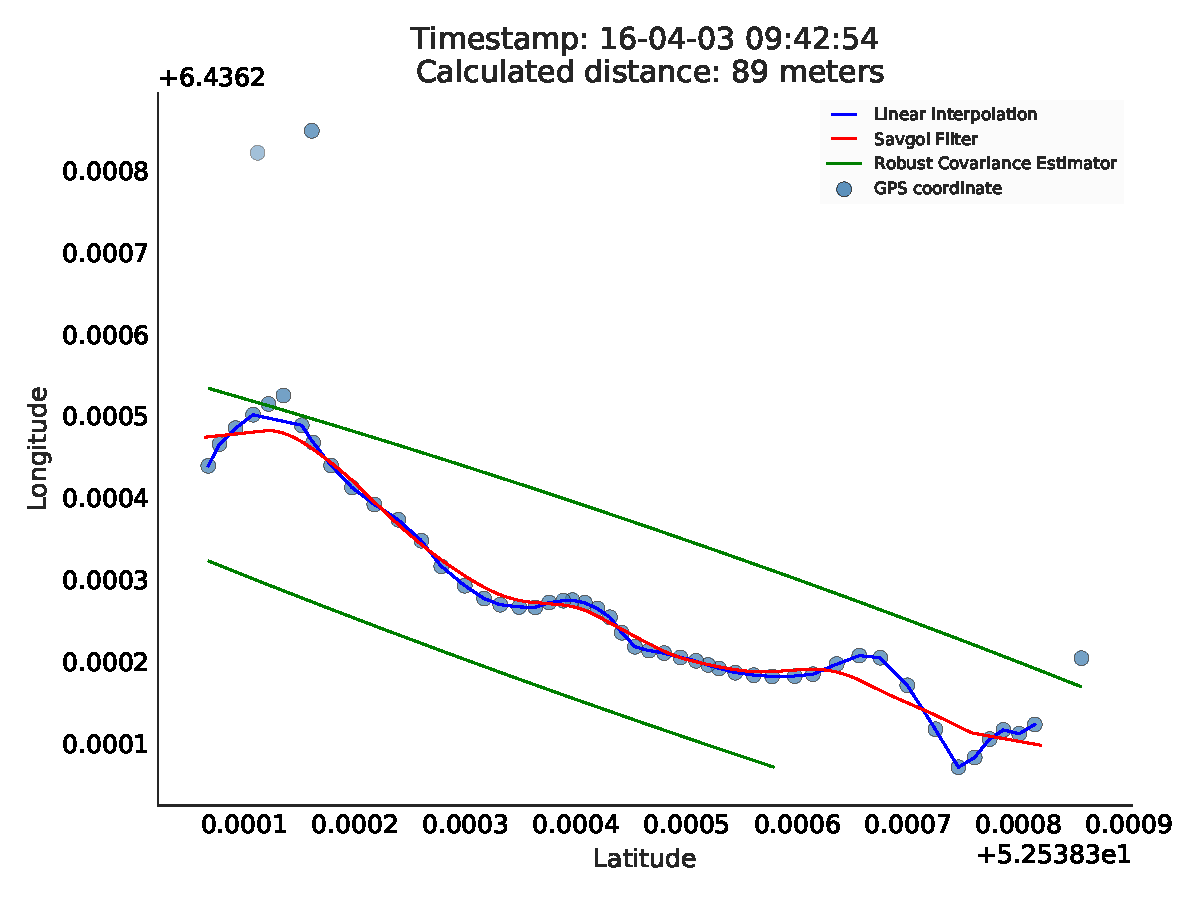
\includegraphics[scale=0.29]{gps/straight/KFb4FtR8Jjb6Ajtdc}
	}
	\vfill
	\subfloat[]{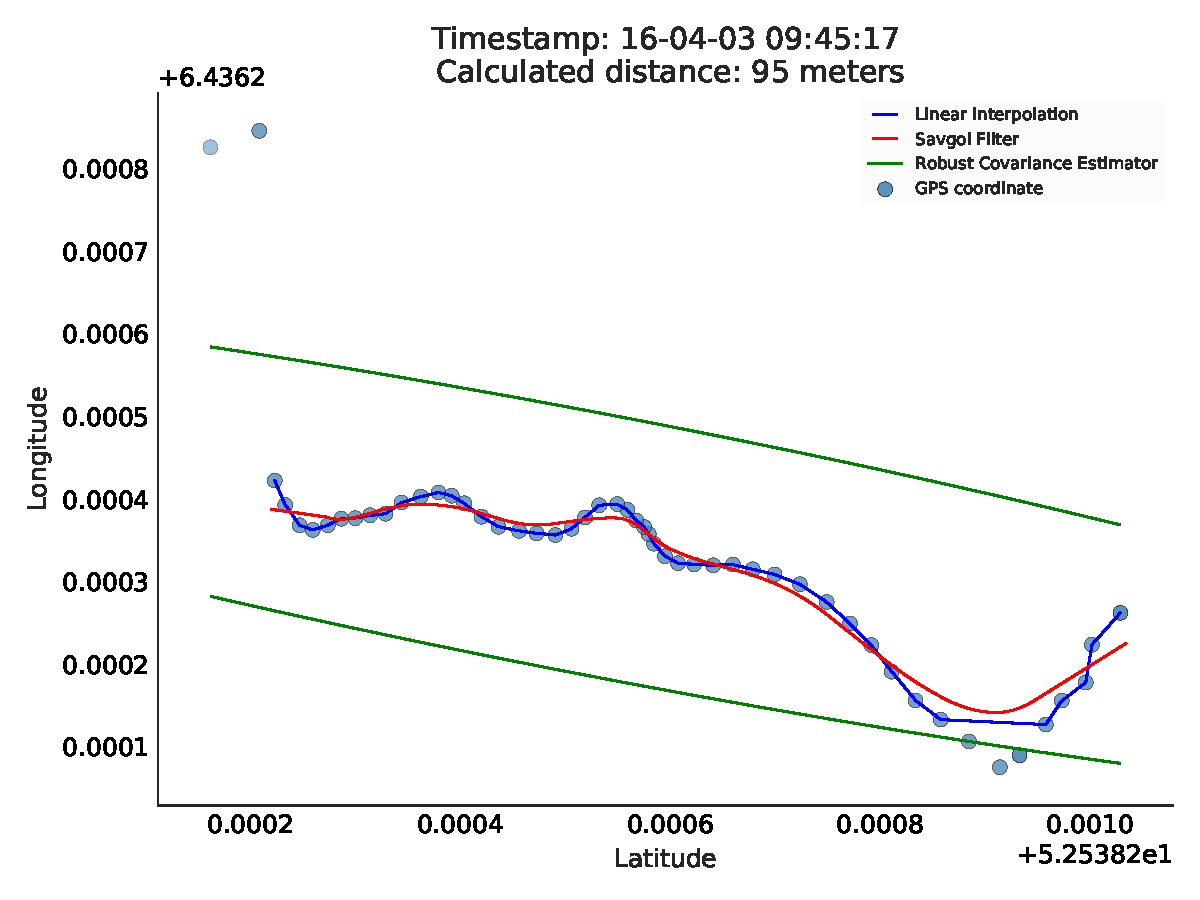
\includegraphics[scale=0.29]{gps/straight/QXtSsihbjmWnG854C}
	}
	\hspace{0.5cm}
	\subfloat[]{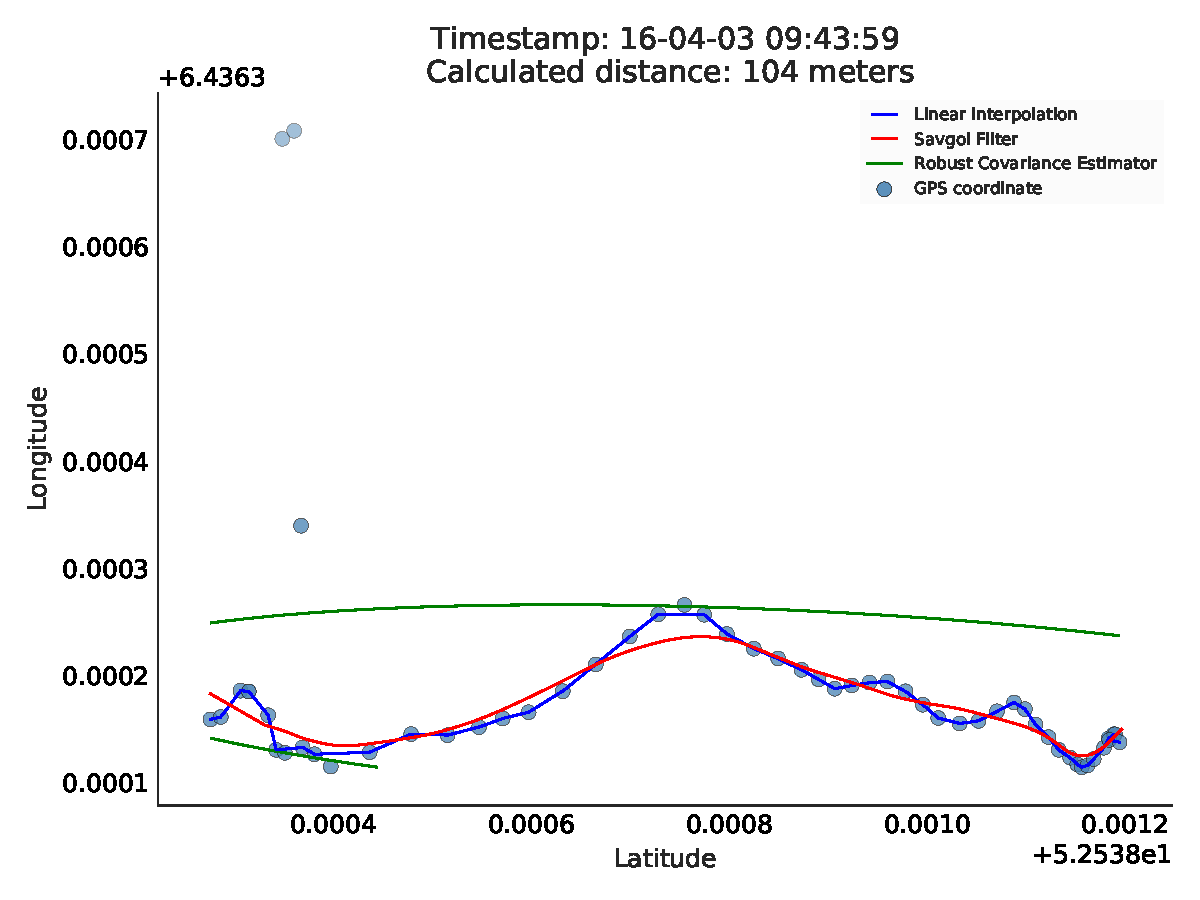
\includegraphics[scale=0.29]{gps/straight/vGn6KLTyNqBEH25YN}
	}
	\captionof{figure}{}
\end{figure}

\newpage

\section{GPS Plots Circular Path}
\begin{figure}[H]
	\centering
	\subfloat[]{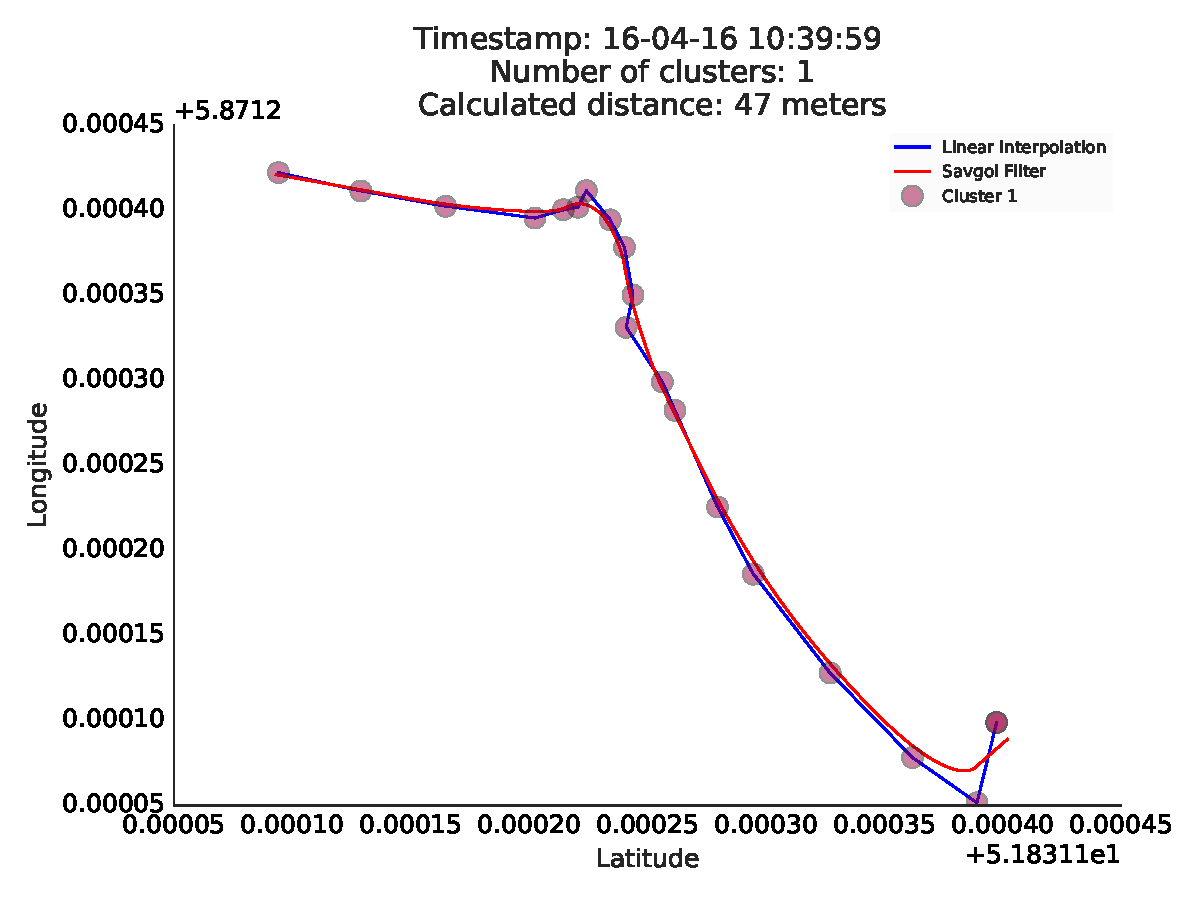
\includegraphics[scale=0.29]{gps/circle/2Zye5dTxYRNq7K7se}
	}
	\hspace{0.5cm}
	\subfloat[]{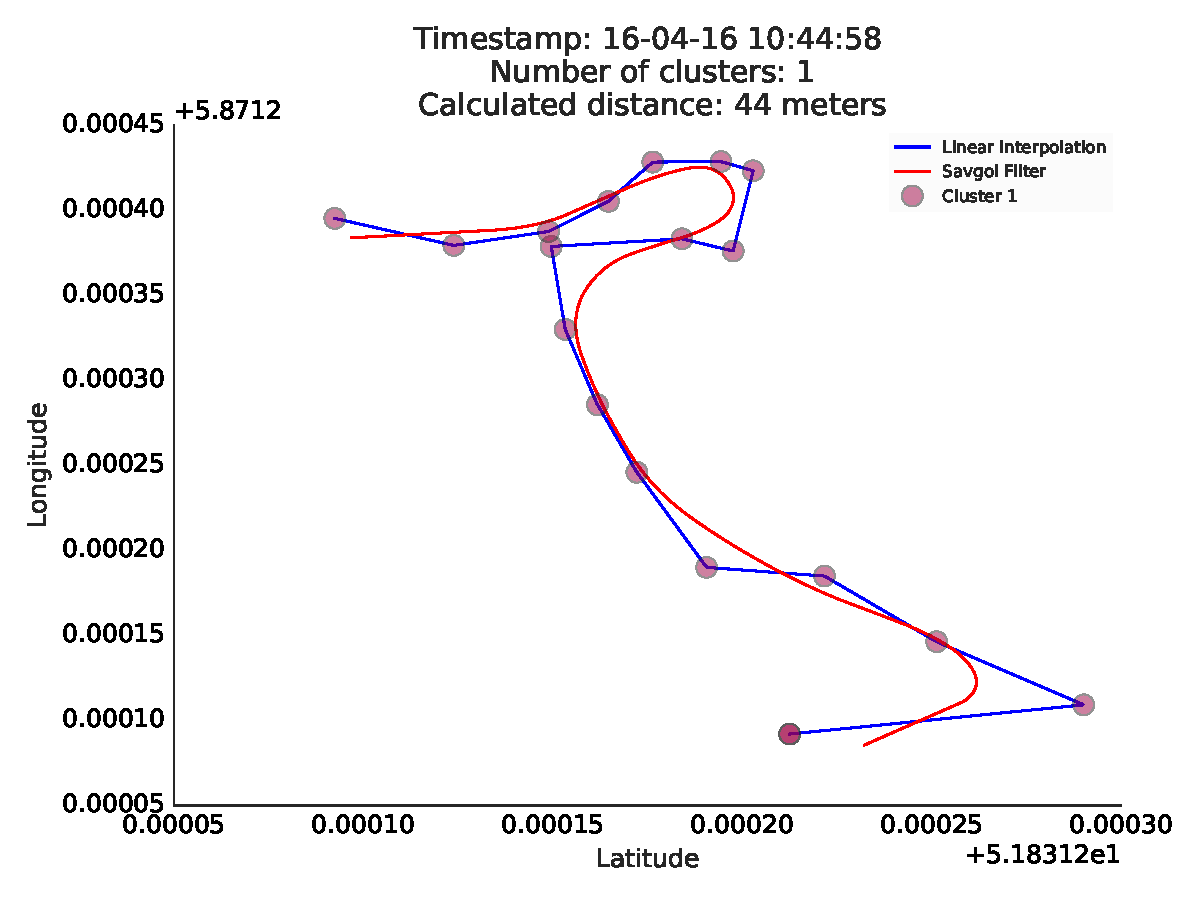
\includegraphics[scale=0.29]{gps/circle/4E2jhxMF392sEjWJF}
	}
	\vfill
	\subfloat[]{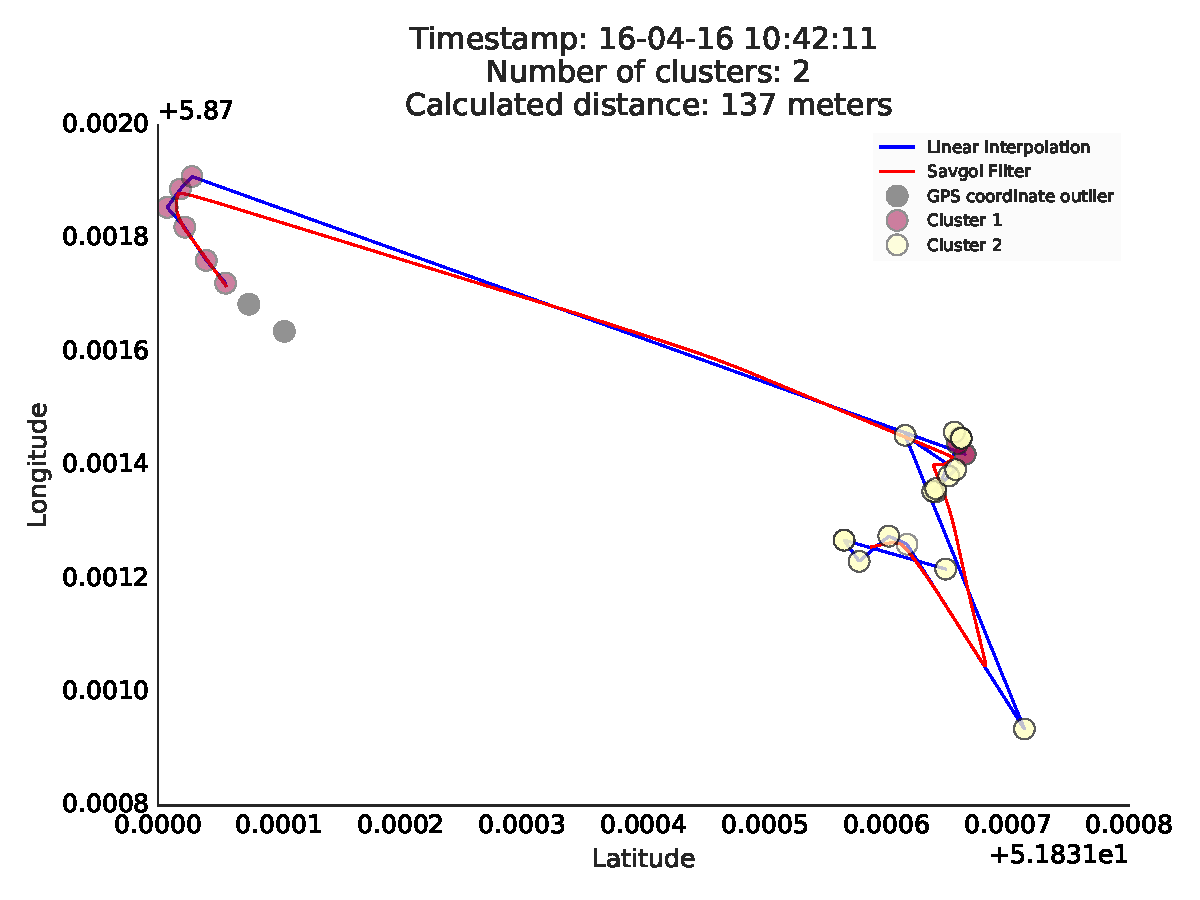
\includegraphics[scale=0.29]{gps/circle/HFgtoEcsXcmiDZHtY}
	}
	% Was eerst 141m door fout, nu 137
	\hspace{0.5cm}
	\subfloat[]{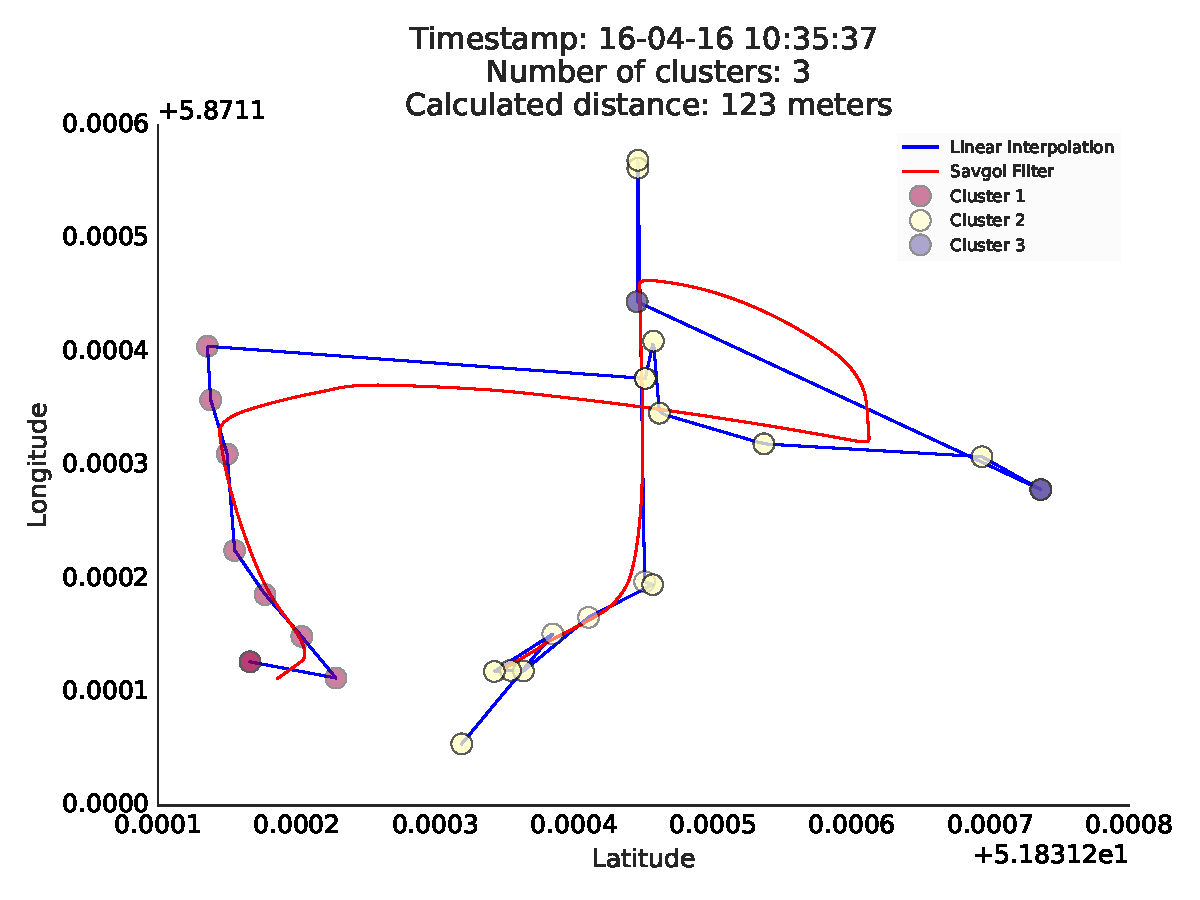
\includegraphics[scale=0.29]{gps/circle/otZE8i4oahYFNdegA}
	}
	\vfill
	\subfloat[]{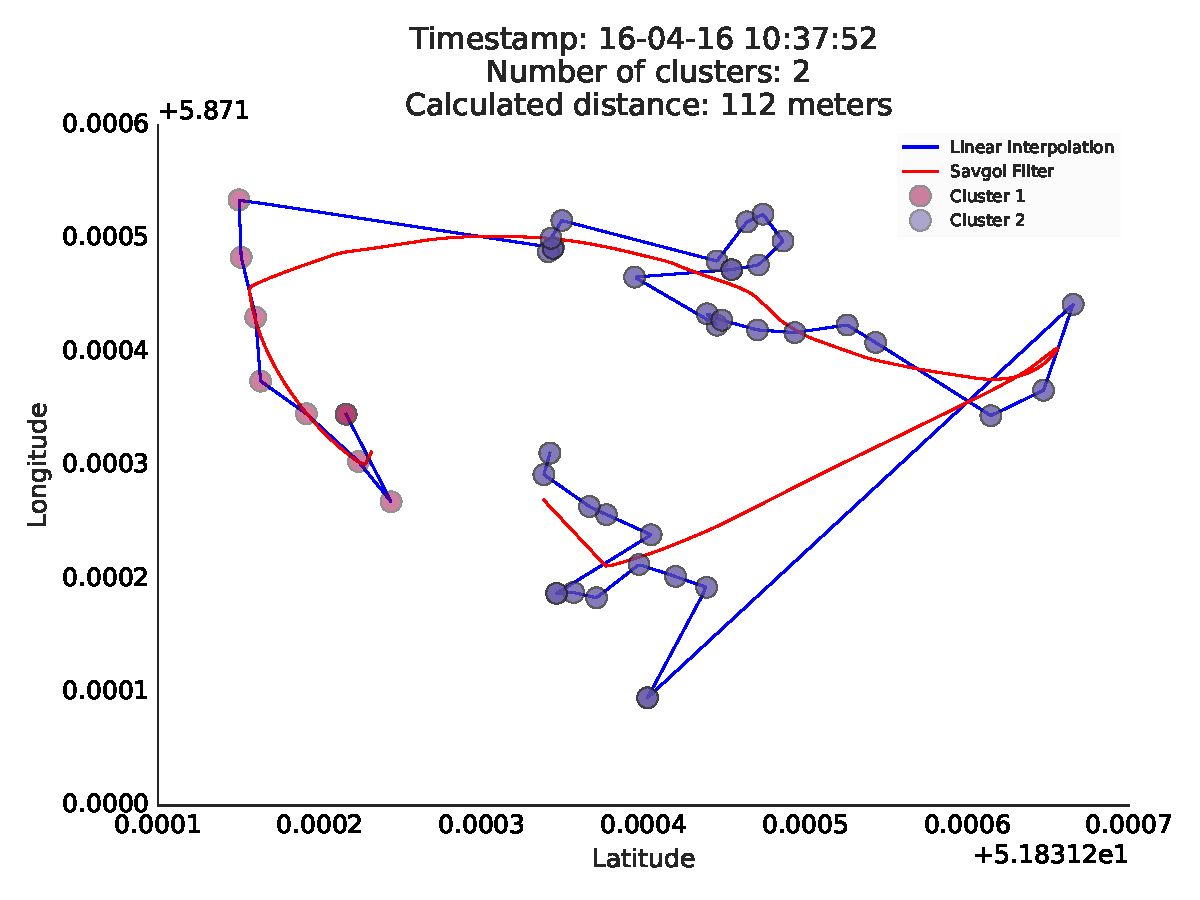
\includegraphics[scale=0.29]{gps/circle/Px5F2nQ9iaYACpJXG}
	}
	\captionof{figure}{Plots of the GPS coordinates of the walking test using a circular track. First, clustering is used to filter out the outliers. Afterwards, inliners are  smoothed in two stages: `Lineair Interpolation' is the first smoothing step and `Savgol Filter' the last. Black points are points classified as noise.}
\end{figure}

\newpage

\section{Heart Rate Boxplots}
\begin{figure}[H]
	\centering
	\subfloat[]{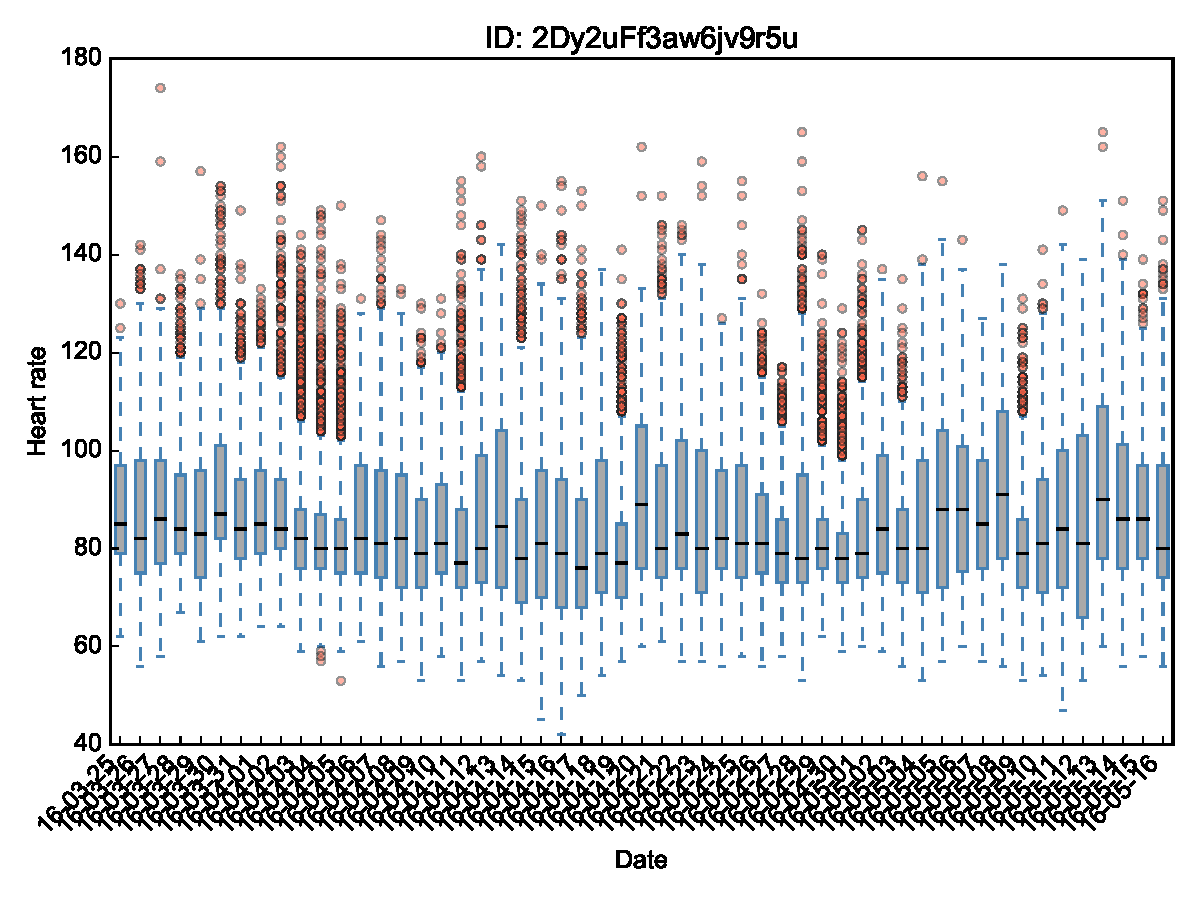
\includegraphics[scale=0.5]{boxplots/2Dy2uFf3aw6jv9r5u}
	}
	\vfill
	\subfloat[]{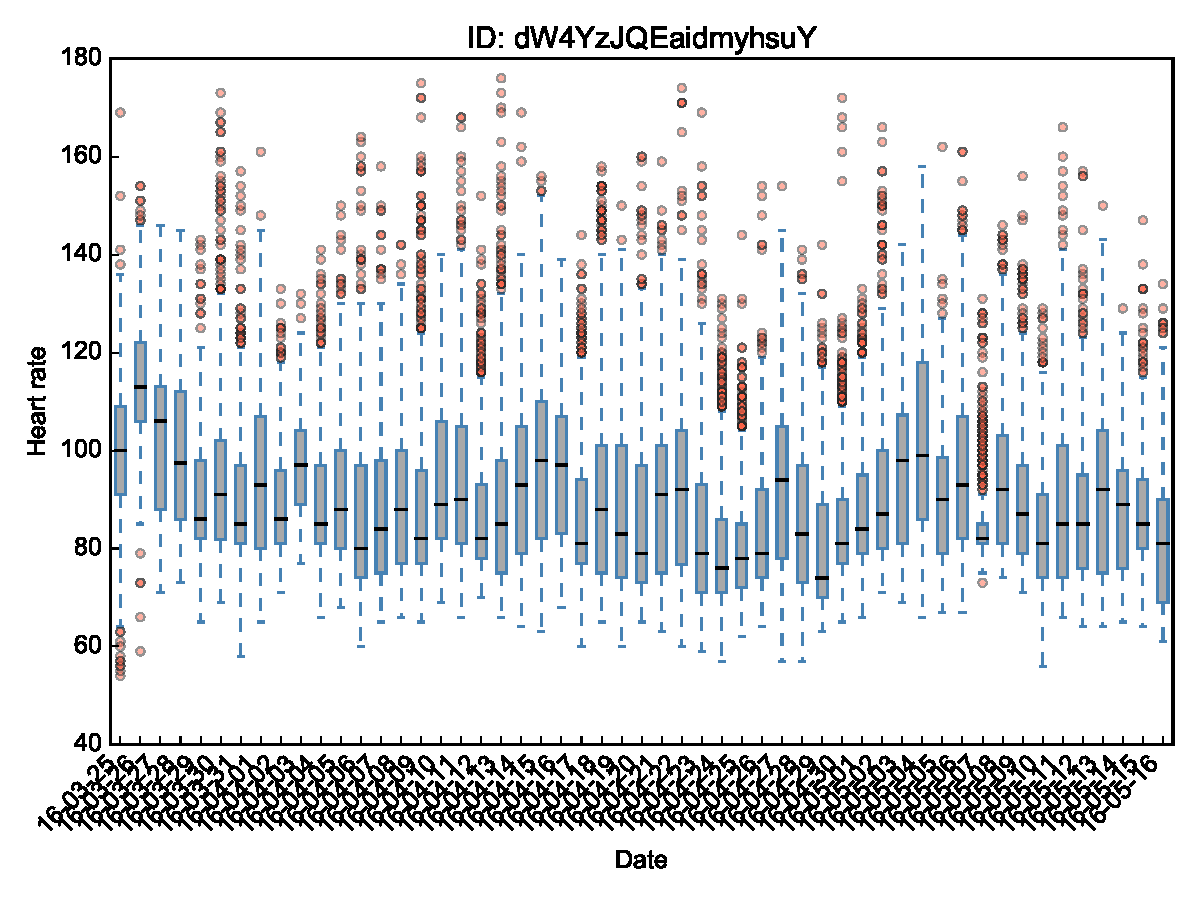
\includegraphics[scale=0.5]{boxplots/dW4YzJQEaidmyhsuY}
	}
	\captionof{figure}{Boxplots of the heart rates for each day.}
	\label{fig: heart rates boxplots}
\end{figure}

\begin{figure}
	\ContinuedFloat
	\centering
	\subfloat[]{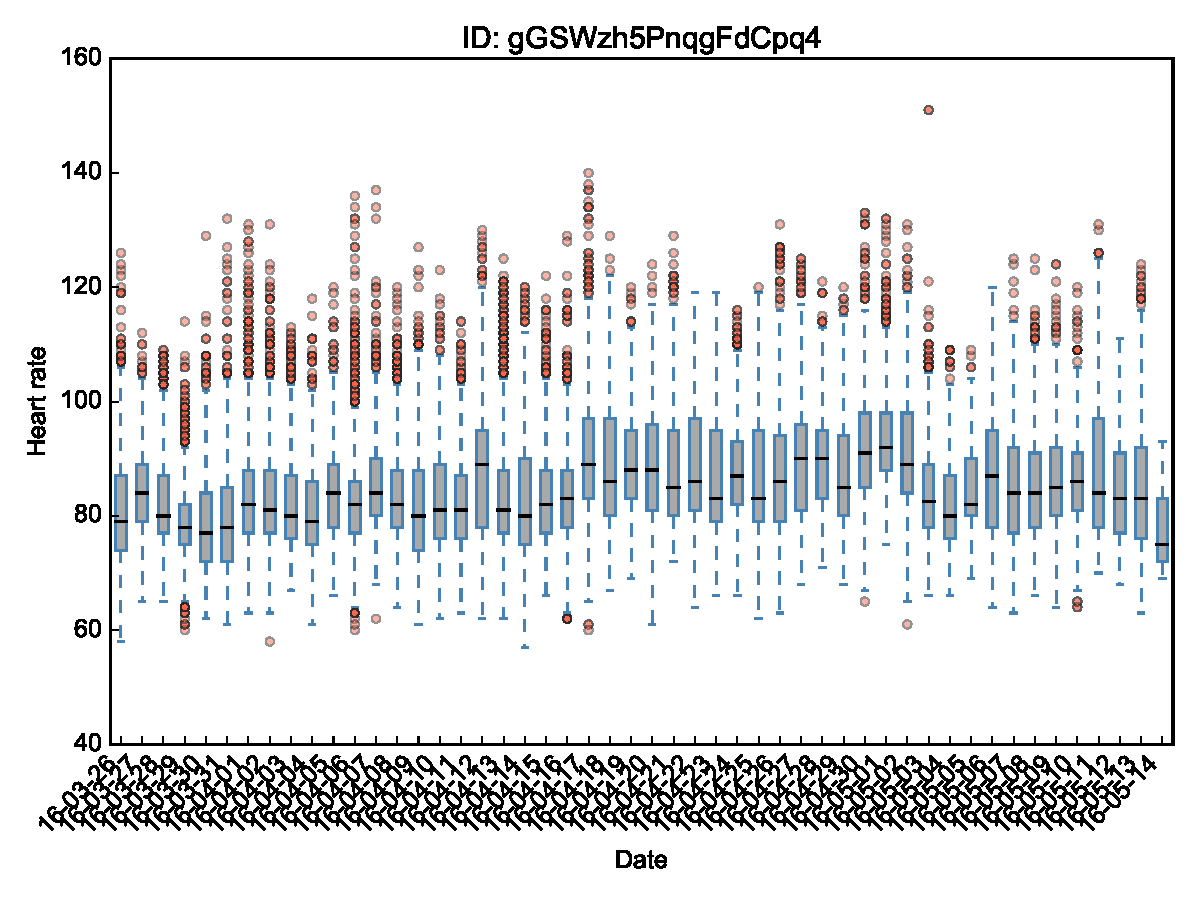
\includegraphics[scale=0.5]{boxplots/gGSWzh5PnqgFdCpq4}
	}
	\vfill
	\subfloat[]{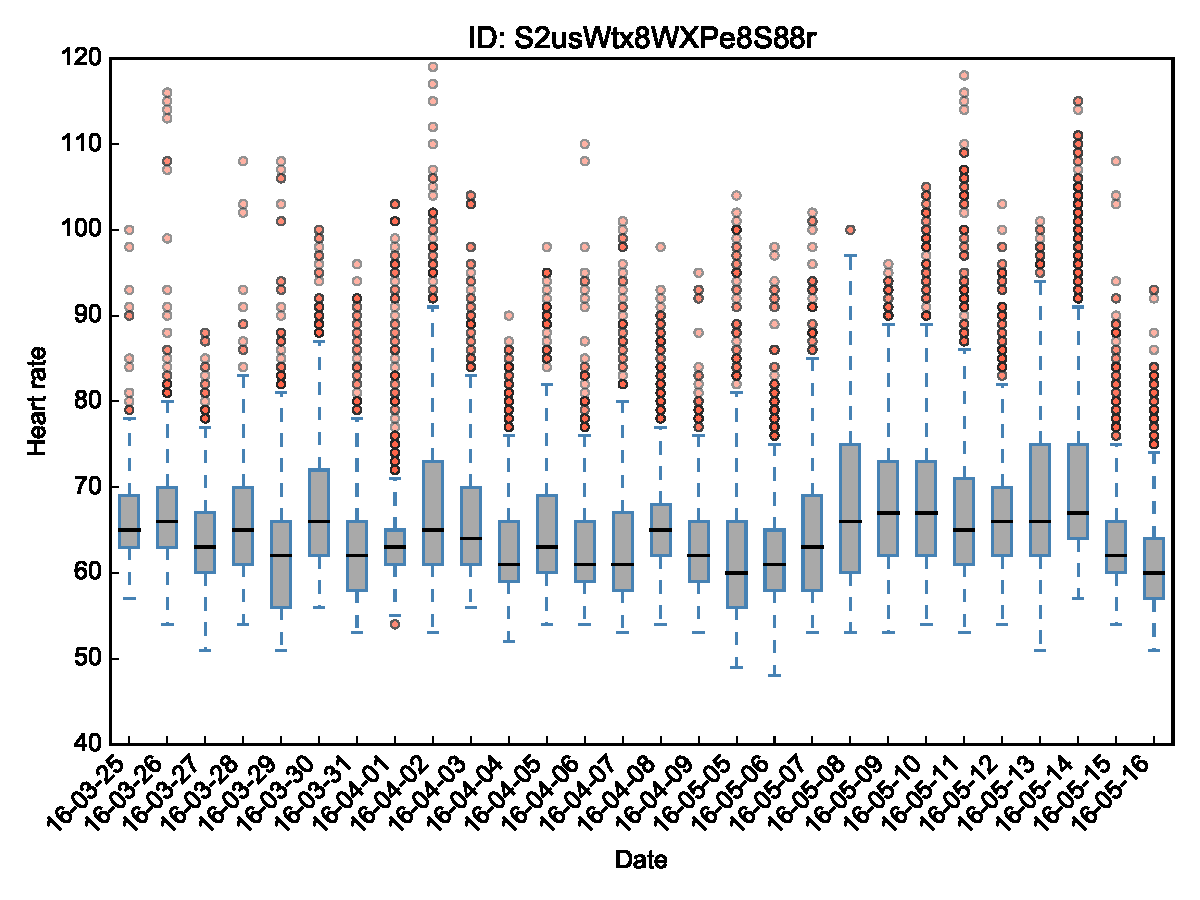
\includegraphics[scale=0.5]{boxplots/S2usWtx8WXPe8S88r}
	}
	\captionof{figure}{}
\end{figure}

\newpage

\section{Elliptic Outlier Detection}
%
\begin{code}
	\begin{minted}[linenos=true, fontsize=\footnotesize, breaklines=true]{python}
def PlotEllipticOutliers(rawPositions, ID, timestmp):
    """
    This method is used for outlier detection on a straight track.
    Uses the EllipticEnvelope object from Scikit-learn
    :param rawPositions:    The raw GPS positions
    :param ID:              The ID of the user
    :param timestmp:        The timestamp
    """
    folder = "out/"
    plotDir = folder + "plots/Walking Test"

    lats = []
    longs = []
    timestamps = []
    for pos in rawPositions:
        lat = pos["latitude"]
        long = pos["longitude"]
        timestamp = pos["timestamp"]
        lats.append(lat)
        longs.append(long)
        timestamps.append(timestamp)

    # writeToFile(ID, "output", lats, longs)
    classifiers = {
        "Robust Covariance Estimator": EllipticEnvelope(contamination=0.08, support_fraction=0.8)
    }
    alpha = 0.5
    linewidth = 0.15

    classifierName = "Robust Covariance Estimator"
    classifier = classifiers[classifierName]
    X = zip(lats, longs)
    xx1, yy1 = np.meshgrid(np.linspace(min(lats), max(lats), 1000), np.linspace(min(longs), max(longs), 1000))
    classifier.fit(X)
    Z1 = classifier.decision_function(np.c_[xx1.ravel(), yy1.ravel()])
    Z1 = Z1.reshape(xx1.shape)
    CS = plt.contour(xx1, yy1, Z1, levels=[0], linewidths=1, colors="g")
    CS.collections[0].set_label(classifierName)
    plt.scatter(lats, longs, s=50, alpha=alpha, linewidth=linewidth, edgecolor=almost_black, color="steelblue",
                label="GPS coordinate")
    plt.autoscale(enable=True, axis="both")
    filteredPositions = []

    for lat, long, timestamp in zip(lats, longs, timestamps):
        z = classifier.decision_function(np.c_[lat, long])
        if z > 0:  # Check if coordinate (lat, long) is within the ellipse
            filteredPositions.append((lat, long, timestamp))

    y = zip(*filteredPositions)[0]  # the latitudes
    x = zip(*filteredPositions)[1]  # the longitudes
    t = zip(*filteredPositions)[2]  # the timestamps

    x2, y2, newx2, newy2 = smooth(y, x, t)
    plt.plot(y2, x2, label="Linear Interpolation")
    totalDistance = calcDistanceWalked(newy2, newx2)

    plt.plot(newy2, newx2, label="Savgol Filter", color="r")
    plt.title("Timestamp: %s\n Calculated distance: %i meters" % (timestmp, totalDistance))
    plt.xlabel("Latitude")
    plt.ylabel("Longitude")
    fancyPlot()
    writeToPdf(ID, plotDir)

\end{minted}
	\caption{Code used for detecting outliers in a straight path.}
	\label{GPS Smoothing Code Straight Line}
\end{code}
%

\newpage

\section{Clustering Outlier Detection}
%
\begin{code}
	\begin{minted}[linenos=true, fontsize=\footnotesize, breaklines=true]{python}
def clustering(lats, longs, timestamps, ID, timestmp, multiPDF=False):
    """
    Clusters the GPS coordinates using DBSCAN
    :param timestmp:                The timestamp
    :param ID:                      The ID
    :param timestamps:              The timestamps of the GPS coordinates
    :param lats:                    The latitudes
    :param longs:                   The longitudes
    :return:                        The rounded distance
    """
    folder = "out/"
    plotDir = folder + "plots/Walking Test Analysis"

    R = 6371  # Radius of the earth in km
    cartesianX = []
    cartesianY = []
    cartesianZ = []

    for lat, long in zip(lats, longs):
        # Convert to cartesian coordinates
        x = R * cos(lat) * cos(long)
        y = R * cos(lat) * sin(long)
        z = R * sin(lat)
        cartesianX.append(x)
        cartesianY.append(y)
        cartesianZ.append(z)

    combined = np.vstack((cartesianX, cartesianY, cartesianZ)).T
    (core_samples, labels) = dbscan(combined, eps=0.5)
    grouped = zip(labels, core_samples)
    nonGroupedPositions = []

    for (label, core_sample) in grouped:
        if label != -1:
            lat = lats[core_sample]
            long = longs[core_sample]
            stamp = timestamps[core_sample]
            nonGroupedPositions.append((lat, long, stamp))

    if len(nonGroupedPositions) > 0:
        y = zip(*nonGroupedPositions)[0]  # the latitudes
        x = zip(*nonGroupedPositions)[1]  # the longitudes
        t = zip(*nonGroupedPositions)[2]  # the timestamps
        x2, y2, newx2, newy2 = smooth(y, x, t)

        plt.plot(y2, x2, label="Linear Interpolation")
        plt.plot(newy2, newx2, label="Savgol Filter", color="r")
        distance = calcDistanceWalked(newy2, newx2)
        grouped = sorted(grouped, key=itemgetter(0))

        clusters = {}
        labels = []
        for key, group in groupby(grouped, key=itemgetter(0)):
            # group the clusters based on their label
            labels.append(key)
            clusters[key] = [el[1] for el in group]

        noise = False
        colors = plt.get_cmap("Spectral")(np.linspace(0, 1, len(clusters)))
        for label in labels:
            indices = clusters[label]
            latitudes = []
            longitudes = []
            size = 10
            alpha = 0.5
            lineWidth = 0.15
            for i in indices:
                latitudes.append(lats[i])
                longitudes.append(longs[i])
            if label == -1:
                # outliers are identified with a label of -1
                plt.plot(latitudes, longitudes, "o", markerfacecolor=almost_black, markeredgecolor=almost_black,
                         markersize=size, alpha=alpha, linewidth=lineWidth, label="Outlier")
                noise = True
            else:
                plt.plot(latitudes, longitudes, "o", markerfacecolor=colors[label], markeredgecolor=almost_black,
                         markersize=size, alpha=alpha, linewidth=lineWidth, label="Cluster %i" % (label + 1))

        plt.title("Timestamp: %s\n Number of clusters: %i\n Calculated distance: %i meters" % (
            timestmp, (len(clusters) - 1) if noise else len(clusters), round(distance)))
        plt.xlabel("Latitude")
        plt.ylabel("Longitude")
        fancyPlot()
        writeToPdf(ID, plotDir)
        return True, distance
    else:
        # DBSCAN gave back an empty array, therefore we cannot perform any smoothing or distance calculation
        return False, 0
\end{minted}
	\caption{Code used for detecting outliers in a non-straight path.}
	\label{GPS Smoothing Code Non-Straight Line}
\end{code}
%

\newpage

\section{Calculation of Walking Speed}
%
\begin{code}
	\input{code/"Walking speed".tex}
	\caption{Code used for calculating the walking speed between GPS coordinates.}
	\label{walk test code snippet}
\end{code}
%


\section{Tables}
\subsection{Sleep}
% !TeX spellcheck = en_US
% !TeX root = ../BachelorThesis.tex

\begin{table}[H]
 	\centering
 	\begingroup
 	\fontsize{6pt}{6pt}
 	\selectfont
 	\subfloat[]{
 		\csvautobooktabular[head to column names, table head=\toprule \bfseries Date & \bfseries Rating & \bfseries Duration (h)\\\midrule]
 		{csv/sleep/2Dy2uFf3aw6jv9r5u.csv}
 		\label{table:sleepduration1}
 	}
 	\hspace{1cm}
 	\subfloat[]{
 		\csvautobooktabular[head to column names, table head=\toprule \bfseries Date & \bfseries Rating & \bfseries Duration (h)\\\midrule]
 		{csv/sleep/dW4YzJQEaidmyhsuY.csv}
 		\label{table:sleepduration2}
 	}
 	\captionof{table}{Measurements of the sleep duration of our participants.} 
	\label{table: Sleep Analysis}
	
	\endgroup
\end{table}

\begin{table}[H]
	\ContinuedFloat
	\centering
 	\begingroup
 	\fontsize{6pt}{6pt}
 	\selectfont
 	\subfloat[]{
 		\csvautobooktabular[head to column names, table head=\toprule \bfseries Date & \bfseries Rating & \bfseries Duration (h)\\\midrule]
 		{csv/sleep/gGSWzh5PnqgFdCpq4.csv}
 		\label{table:sleepduration3}
 	}
 	\hspace{1cm}
 	\subfloat[]{
 		\csvautobooktabular[head to column names, table head=\toprule \bfseries Date & \bfseries Rating & \bfseries Duration (h)\\\midrule]
 		{csv/sleep/S2usWtx8WXPe8S88r.csv}
 		\label{table:sleepduration4}
 	}
 	\captionof{table}{}
	\endgroup
\end{table}
\subsection{Heart Rate}
\input{tables/"heart rate"}
\subsection{Walking Test}
\input{tables/"walking test"}



\end{document}